\section{Notes On Emotion Theories With Respect to High-Level Requirements and
Emotion Theories}\label{chapter:reqsTheoryNotes}
% This is a copy of the information from the thesis, modified to work with the
%SRS

These are the notes created about emotion theories with respect to high-level
requirements during analysis (Section~\ref{sec_theories}).
Tables~\ref{tab:theory-req-sys-summary-flexibility},
\ref{tab:theory-req-sys-summary-easeofuse},
\ref{tab:theory-req-comp-summary-flexibility}, and
\ref{tab:theory-req-comp-summary-easeofuse} summarize the resulting scores.

A reminder that the scores are somewhat subjective, and depend on one's
understanding of the requirements and current state of emotion literature.

\subsection{Discrete Theories}
The discrete theories are the most likely candidates for satisfying high-level
requirements that depend on understanding what emotion an NPC has, as this is
their core focus. This includes the flexibility requirements for
\textit{Allowing the Integration of New Components} (\ref{flexNew}) and
\textit{Choosing Which NPC Emotions to Use} (\ref{flexEm}), and the ease-of-use
requirements for \textit{Having a Clear API (Output)} (\ref{easeAPI}) and
\textit{Showing That Emotions Improve the Player Experience} (\ref{easePX}).

\subsubsection{Flexibility: Allowing the Integration of New Components
    (\ref{flexNew})}
All three discrete theories provide variable levels of native support for
personality, but only Plutchik does not touch on mood. None of them touch on
core affect.

\begin{itemize}
    \item \textbf{Ekman \& Friesen} (\weak)
    \begin{itemize}
        \item Moods and personality are inferred from emotion
        signals (e.g. many \textit{Joy}-related signals could suggest a
        cheerful mood)~\citep[p.~48, 55--56]{ekman1999basic}

        \item Little information beyond these definitions $\rightarrow$
        developers would need to create patterns of emotions for each mood and
        trait, could become too time consuming and error-prone

        \item No coverage of Core Affect, Personality and Mood are error-prone
        and time consuming
    \end{itemize}

    \item \textbf{Izard} (\weak)
    \begin{itemize}
        \item Natively accounts for personality
        (\citepg{izard2000motivational}{253--254}; \citepg{izard1977human}{44})
        \begin{itemize}
            \item Emergent phenomena that begins at birth and develops as the
            individual interacts with their environment

            \item Treated as a product of emotions associated with patterns in
            perception, cognition, and behaviour

            \item [$\rightarrow$] Requires developers to create patterns for
            each personality trait, which is likely to be too time consuming
            and error-prone
        \end{itemize}

        \item Seems to acknowledge two definitions of mood
        \begin{itemize}
            \item Defined as a ``continuing total life condition'' similar to
            what he calls an emotion trait, or tendencies towards certain
            emotion experiences~\citep[p.~17, 171]{izard1991psychology}
            $\rightarrow$ in the view of stable traits and fluid states,
            conceptualization appears to be closer to personality than mood

            \item As a state, defined as an enduring emotion state that is too
            mild to enter conciousness but can influence mental health and
            bodily systems, such as the immune
            system~\citep[p.~21]{izard1991psychology} $\rightarrow$ closer to
            working definition of mood in \progname{}'s context

            \item [$\rightarrow$] could be realized as a timed function that
            monitors an NPC's emotion state and acts on those that have not
            surpassed a given threshold (minimal effort to implement)
        \end{itemize}

        \item No coverage of Core Affect, Mood requires minimal effort,
        Personality is error-prone and time consuming
    \end{itemize}

    \item \textbf{Plutchik} (\good)
    \begin{itemize}
        \item Natively accounts for personality
        \begin{itemize}
            \item Connects its emotion circumplex directly to a
            circumplex of personality traits\footnote{The assumption that
                the circumplexes can be connected this way might be naive. They
                might be unique to the modelled domain rather than showing
                similarities across them~\citep[p.~815]{feldman1995variations}.}
            \citep[p.~27--28]{plutchik1997circumplex} $\rightarrow$ could
            mechanize with a simple weighting mechanism such that emotions are
            easier or harder to elicit

            \item Built around a layperson's understanding of personality
            $\rightarrow$ upholds the \textit{Hiding the Complexity of Emotion
                Generation} (\ref{easeHide}) requirement
        \end{itemize}

        \item circumplex is a way to incorporate a model of mood
        \begin{itemize}
            \item Agreement that it can be represented by an elliptical
            circumplex with arousal as the shorter
            dimension~\citep[p.~806, 812, 814]{feldman1995variations}

            \item Could add an additional element such that the length of the
            arousal dimension changes with context $\rightarrow$ afford
            more creative freedom than a fixed model

            \item Can uphold the \textit{Hiding the Complexity of Emotion
                Generation} requirement (\ref{easeHide}) with a well-designed
            interface, with details available for advanced users
        \end{itemize}

        \item Dimensional nature of theory could aid in a non-native
        representing core affect $\rightarrow$ could map the intensity
        dimension to arousal and the relative positions of an emotion to
        some anchor points as \textit{valence}
        \begin{itemize}
            \item Mapping might not be understandable due to debate about the
            \textit{valence} of \textit{Surprise} and its relation to
            \textit{Anticipation}~\citep[p.~98]{susanto2020hourglass}
            $\rightarrow$ concessions could be made, such as listing some
            categories as zero \textit{valence}, since \progname{} is
            unconcerned with realism

            \item Can uphold the \textit{Hiding the Complexity of Emotion
                Generation} requirement (\ref{easeHide}) with a well-designed
            interface, with details available for advanced users
        \end{itemize}

        \item Ability to build \textit{some} type of Core Affect and Mood
        representation on top of existing theory, Personality native to theory
        and built on a layperson's perspective
    \end{itemize}
\end{itemize}

\subsubsection{Flexibility: Choosing What Emotions the NPC can Have
(\ref{flexEm})}
Within each discrete theory's set of emotions, it would be easy to exclude any
of them if they are not needed. However, \textit{adding} more emotions to a set
is less clear cut. There does not seem to be any convincing empirically
validated or verifiable rules for creating ``non-basic'' emotions in discrete
theories~\citep[p.~6]{ortony2021all}. This does not impact \progname{} because
it does not need to replicate true affective phenomena---it need only produce
convincing results.

\begin{itemize}
    \item \textbf{Ekman \& Friesen} (\weak)
    \begin{itemize}
        \item Do not believe that there are ``non-basic''
        emotions~\citep[p.~55, 57]{ekman1999basic}
        \begin{itemize}
            \item Each emotion represents a family of related states that share
            a theme, and variations between members are the result of learning

            \item [$\rightarrow$] Requires developers to either associate
            different situations for the desired variations manually or create
            a learning mechanism to create them as the NPC interacts with the
            game environment

            \item Unideal $\rightarrow$ Could be difficult to adapt this kind
            of system to simple games, violating the \textit{Ability to Operate
                on Different Levels of NPC Complexity} requirement
            (\ref{flexComplex}); requires some knowledge of psychology and
            neuroscience, violating the \textit{Hiding the Complexity of
                Emotion Generation} (\ref{easeHide}) requirement
        \end{itemize}

        \item Facial expressions can be blends of prototypical primary
        ones~\citep[p.~69]{ekman2007emotions}
        \begin{itemize}
            \item Step removed from the emotion generation process, and would
            likely happen in an emotion expression component

            \item Would need to translate the blended expression into an
            emotion to use it for emotion generation $\rightarrow$ feasible,
            but error-prone, method as facial expression interpretations can be
            subjective
        \end{itemize}

        \item No ``non-basic'' emotions, translating from facial expressions is
        error-prone
    \end{itemize}

    \item \textbf{Izard} (\disqualified)
    \begin{itemize}
        \item ``New emotions'' are the product of affective-cognitive
        structures~\citep[p.~564--565]{izard1992basic}
        \begin{itemize}
            \item Association of primary emotion patterns or clusters with
            images, thoughts, and memories

            \item [$\rightarrow$] Requires developers to either create these
            structures manually or create a learning mechanism to create them
            as the NPC interacts with the game environment

            \item Unideal $\rightarrow$ Same reasons as Ekman \& Friesen,
            violating both the \textit{Ability to Operate on Different Levels
                of NPC Complexity} and \textit{Hiding the Complexity of Emotion
                Generation} requirements (\ref{flexComplex}, \ref{easeHide})
        \end{itemize}

        \item Difficult to adapt to different NPC complexities, requires
        knowledge for connecting emotions to cognitive patterns
    \end{itemize}

    \item \textbf{Plutchik} (\strong)
    \begin{itemize}
        \item One of the better developed theories of emotion mixes
        (\citepg{ledoux1996emotional}{113}; \citepg{ortony2021all}{3, 5})

        \item Might be the only discrete theory to focus on this aspect of the
        ``primary'' emotions~\citep[p.~47]{ekman1999basic}

        \item Colour wheel analogy uses concepts and terms that are generally
        understood by laypeople $\rightarrow$ does not require any knowledge of
        the theory to use
        \begin{itemize}
            \item Lacks clarity about technical rules for combining emotions
            (\citepg{johnson1992basic}{208--209}; \citepg{ortony2021all}{5})
            \textbf{BUT} laypeople tend to attribute the same underlying
            primary emotions to named emotions outside the primary
            set~\citep[p.~204--205]{plutchik1984emotions}

            \item [$\rightarrow$] Implies that a game developer can apply their
            own experiences when deciding how to represent a new emotion with
            the Plutchik circumplex
        \end{itemize}

        \item Ability to build additional emotions from existing set, based on
        a layperson's understanding of emotions and their combinations
    \end{itemize}
\end{itemize}


\subsubsection{Ease-of-Use: Having a Clear API (Output)  (\ref{easeAPI})}
The discrete theories are generally easy for laypeople to understand. All three
theories connect their emotions to distinctive behaviours that can be applied
to situations of variable complexity. This makes for a clean output API,
providing an emotion category that developers can attach to ``buckets'' of
related behaviours and expressions that are ``familiar''.

\begin{itemize}
    \item \textbf{Ekman \& Friesen} (\strong)
    \begin{itemize}
        \item Have publications that are meant for the general public (e.g.
        \cite{ekman2007emotions}) $\rightarrow$ accessible to laypeople

        \item Use of facial expressions is a helpful tool for conveying meaning
        about their primary emotions
    \end{itemize}

    \item \textbf{Izard} (\weak)
    \begin{itemize}
        \item Gains understandability by connecting its emotions to facial
        expressions, although some emotions are not connected to one

        \item [$\rightarrow$] Weakens its usability, as some developers might
        actively avoid the emotions that cannot be readily represented on the
        face
    \end{itemize}

    \item \textbf{Plutchik} (\good)
    \begin{itemize}
        \item Construction based on similarities and differences between
        affective terms as they are understood in (English) language
        $\rightarrow$ can help developers understand each emotion based on
        their understanding of the word's meaning and its relative position to
        other emotion words on the circumplex

        \item Each primary emotion is also connected to an intended behaviour
        pattern, like rejection and
        exploration~\citep[p.~202]{plutchik1984emotions}
        \begin{itemize}
            \item  Addresses problems of ``missing'' facial expressions with
            characteristic or typical behaviours
            (\citepg{julle2020there}{20--21};
            \citepg{schindler2013admiration}{101})

            \item [$\rightarrow$] Could help developers conceptualize what each
            emotion could look and act like, can include facial expressions
        \end{itemize}

        \item Does not directly benefit from assigned facial expressions, but
        some connections could be made with Ekman \& Friesen and Izard
        (Table~\ref{tab:discreteEmotions}) $\rightarrow$ understanding of
        emotion terms and associated behaviours is not as ``clear cut''
    \end{itemize}
\end{itemize}

\begin{table}[!tb]
    \begin{center}
        \renewcommand{\arraystretch}{1.2}
        \begin{threeparttable}
            \caption{Primary Emotions in Discrete Theories}
            \label{tab:discreteEmotions}

            \begin{tabular}{lccc}
                \toprule
                \textbf{Emotion} & {\begin{tabular}[c]{@{}c@{}}\textbf{Ekman \&
                            Friesen} \\
                        \textbf{\citep{ekman2007emotions}}\end{tabular}} &
                \textbf{\citet{izard1993stability}} &
                \textbf{\citet{plutchik1997circumplex}} \\ \hline

                \rowcolor[gray]{0.9}Happiness/Enjoyment/Joy\textsuperscript{\large\Jupiter\Pluto}
                & \checkmark & \checkmark & \checkmark \\

                Sadness\textsuperscript{\large\Jupiter\Pluto} & \checkmark &
                \checkmark & \checkmark \\

                \rowcolor[gray]{0.9}Fear\textsuperscript{\large\Jupiter\Pluto}
                & \checkmark & \checkmark & \checkmark \\

                Anger\textsuperscript{\large\Jupiter\Pluto} & \checkmark &
                \checkmark & \checkmark \\

                \rowcolor[gray]{0.9}Surprise\textsuperscript{\large\Jupiter\Pluto}
                & \checkmark & \checkmark & \checkmark \\

                Disgust\textsuperscript{\large\Jupiter\Pluto} & \checkmark &
                \checkmark &
                \checkmark \\

                \rowcolor[gray]{0.9}Contempt\textsuperscript{{\normalsize\Moon}{\large\Pluto}}
                & \checkmark & \checkmark &
                {\small\textpmhg{\Hibp}} \\

                Interest\textsuperscript{\large\Pluto} &  & \checkmark &
                \checkmark \\

                \rowcolor[gray]{0.9}Guilt\textsuperscript{\large\textpmhg{\Hl}}
                 & & \checkmark & {\small\textpmhg{\Hibp}} \\

                Shame\textsuperscript{\large\Pluto} &  & \checkmark &
                {\small\textpmhg{\Hibp}} \\

                \rowcolor[gray]{0.9}Shyness\textsuperscript{\large\Pluto}
                &  & \checkmark & \\

                Acceptance\textsuperscript{{\large\textpmhg{\Hl}}\textpmhg{\Hi}}
                &  & & \checkmark \\
                \hline

                \bottomrule

            \end{tabular}

            \begin{tablenotes}
                \footnotesize
                \vspace*{2mm}

                \item []{\Large\Jupiter} \textit{Associated with a facial
                    expression by \citet{ekman2003unmasking}.}

                \item []{\Large\Pluto} \textit{Associated with a facial
                    expression by \citet[p.~236--237]{izard1971face},
                    \citet[p.~85--91]{izard1977human}.}

                \item []{\normalsize\Moon} \textit{Associated with a facial
                    expression by \citet[p.~184--186]{ekman2007emotions}.}

                \item []{\normalsize\textpmhg{\Hibp}} \textit{As a mixture of
                    the primary emotions.}

                \item []{\normalsize\textpmhg{\Hl}} \textit{Might not have a
                characteristic expression
                    (\citepg{keltner1996evidence}{155};
                    \citepg{schindler2013admiration}{106}), but artistic
                    renditions of facial expressions exist (e.g.
                    \citet{lebrun1760admiration}).}

                \item []{\normalsize\textpmhg{\Hi}} \textit{Plutchik is noted
                as the only researcher to consider \textit{Adoration}---the
                highest intensity of \textit{Acceptance}---a primary
                emotion~\citep[p.~87--88]{schindler2013admiration}.}

                \vspace*{-7mm}
            \end{tablenotes}
        \end{threeparttable}%
    \end{center}
\end{table}

\subsubsection{Ease-of-Use: Showing that Emotions Improve the Player Experience
    (\ref{easePX})}
Like the \textit{Having a Clear API (Output)} requirement  (\ref{easeAPI}),
discrete theories are generally understandable by laypeople. This helps
identify ways to design studies to evaluate and ways to build the player
experience.

\begin{itemize}
    \item \textbf{Ekman \& Friesen} (\good)
    \begin{itemize}
        \item Emotions could be directly connected to an expression module
        built on the Facial Action Coding System (FACS), which is part of the
        theory itself~\citep{facs}

        \item Players could report on their experiences based on NPC
        expressions $\rightarrow$ relatively easy to test how emotions impact a
        player, but limited to facial expressions alone
    \end{itemize}

    \item \textbf{Izard} (\good)
    \begin{itemize}
        \item Considerable overlap between Ekman \& Friesen and Izard regarding
        facial expressions~\citep[p.~3]{ekman2007emotions} $\rightarrow$ could
        be connected to an emotion expression component built on FACS, probably
        with minimal effort

        \item Players could report on their experiences based on NPC
        expressions $\rightarrow$ relatively easy to test how emotions impact a
        player, but limited to facial expressions alone
    \end{itemize}

    \item \textbf{Plutchik} (\good)
    \begin{itemize}
        \item Could be connected to facial expressions, but there is no obvious
        match for \textit{Acceptance} emotion type

        \item Associates each emotion with a behaviour that could be applied to
        a number of actions and expressions that an NPC could need
        $\rightarrow$ design studies around these behaviour classes

        \item Players could report on their experiences based on NPC
        expressions $\rightarrow$ relatively easy to test how emotions impact a
        player, but likely an element of subjectivity in matching behaviours to
        meaning
    \end{itemize}
\end{itemize}

\subsubsection{Examining the Remaining Requirements}
The absence of a defined emotion elicitation tasks in the discrete theories is
a double-edged sword---some requirements are trivial to satisfy, while others
are impossible. The lack of elicitation processes makes it impossible for
discrete theories to satisfy most task-related requirements---they simply do
not exist. This means that they \textit{cannot} be categorized for the
component-level requirements
(Tables~\ref{tab:theory-req-comp-summary-flexibility} and
\ref{tab:theory-req-comp-summary-easeofuse}). For the remaining system-level
requirements (Tables~\ref{tab:theory-req-sys-summary-flexibility} and
\ref{tab:theory-req-sys-summary-easeofuse}), the theories satisfy the
requirements in similar ways, so they are examined as a single unit.
\begin{itemize}
    \item \textit{Flexibility: Independence from an Agent Architecture
        (\ref{flexArch})} (\good)
    \begin{itemize}
        \item No specific tasks $\rightarrow$ effectively architecture-agnostic

        \item Only require processes that satisfy input and output requirements
    \end{itemize}

    \item \textit{Flexibility: Allowing Developers to Specify How to Use
        Outputs (\ref{flexOut})} (\good)
    \begin{itemize}
        \item No specific tasks $\rightarrow$ affords flexibility for
        specifying how to use \progname{}'s outputs

        \item Theoretically could hook up any process to \progname{} using the
        emotions as ``buckets'' for collecting related behaviours
    \end{itemize}

    \item \textit{Flexibility: Ability to Operate on Different Levels of NPC
        Complexity (\ref{flexComplex})} (\good)
    \begin{itemize}
        \item Could add processes and parameters as needed $\rightarrow$ does
        not affect core \progname{} processes
    \end{itemize}

    \item \textit{Flexibility: Be Efficient and Scalable (\ref{flexScale})}
    (\good)
    \begin{itemize}
        \item Could add processes and parameters as needed $\rightarrow$ does
        not affect core \progname{} processes
    \end{itemize}

    \item \textit{Ease-of-Use: Providing Examples of Novel Game Experiences
        (\ref{easeNovel})} (\weak)
    \begin{itemize}
        \item No immediately obvious features for novel game mechanics,
        challenges, or other elements
    \end{itemize}
\end{itemize}

\subsection{Dimensional Theories}
The dimensional theories are the most likely candidates for satisfying
requirements related to CME expansion, as they aim to discover the structure of
emotion and how they relate to other mental
states (\citepg{reisenzein2013computational}{250};
\citepg{broekens2021emotion}{353}). This mainly concerns the flexibility
requirements for \textit{Allowing the Integration of New Components}
(\ref{flexNew}) and \textit{Choosing What Emotions the NPC can Have}
(\ref{flexEm}).

For this analysis, the V-A model is treated as a circumplex as it is a
reasonable representation of affective
states~\citep[p.~296]{remington2000reexamining}, and is more consistent with
affective structure~\citep[p.~12]{barrett1999structure}. The circumplex
also tends to form regardless of the data collected, research domain, and
analysis~\citep[p.~211]{russell1997how}. This representation is not perfect.
There are still issues, such as inclusion/exclusion of terms, self-report
weaknesses, and the effect of context on state
positions~\citep[p.~298]{remington2000reexamining}. However, it also provides
more structure to an otherwise two-dimensional and nebulous space.

\subsubsection{Flexibility: Choosing What Emotions the NPC can Have
(\ref{flexEm})}
Neither V-A or PAD strictly enforce the inclusion of specific emotion types.
Instead, the use of dimensions allows for an infinite number of affective
states. While this trivially supports the ability to \textit{Choose What
    Emotions the NPC can Have} (\ref{flexEm}), it might not be practical for
\progname{} on its own. Instead, adding specific emotions is guided by point
locations representing named emotions. This removes the burden of deciding
where an emotion is located in dimensional space from game designers.

\begin{itemize}
    \item \textbf{V-A} (\weak)
    \begin{itemize}
        \item Space represented by \textit{valence} and \textit{arousal} only
        represents part of an emotion episode (\citepg{yik2002relating}{90};
        \citepg{roseman2011emotional}{441}; \citepg{lisetti2015and}{97})

        \item Unideal $\rightarrow$ some emotions, like \textit{Anger} and
        \textit{Fear}, are difficult to differentiate without additional
        information
        \begin{itemize}
            \item Might be some of the most common emotions that a game
            designer will use $\rightarrow$ could be the \textit{only} two
            emotions required in some games (e.g. NPCs in oppositional
            First Person Shooters (FPSs) due to the game's pace and the
            limited time and ways that players interact with them)
        \end{itemize}

        \item Adding new emotions cannot be adequately contained in V-A
    \end{itemize}

    \item \textbf{PAD} (\good)
    \begin{itemize}
        \item Accompanied by a list of 151 emotion
        labels~\citep[p.~42--45]{mehrabian1980basic} identified from empirical
        data $\rightarrow$ notes their average location in PAD space and the
        standard deviation in the data

        \item List is still finite and cannot account for cultural differences,
        might not cover all of the affective states that a game designer needs
        $\rightarrow$ list is long enough that there is a reasonable chance
        that a game designer can find all the affective state labels that they
        require

        \item Prone to interpretation errors, as the designer's definition and
        the definition used to locate points in PAD space might not be the same
        $\rightarrow$ designers can make their own judgements of the
        suitability of a term based on its coordinates, potentially violating
        \textit{Hiding the Complexity of Emotion Generation} (\ref{easeHide})
    \end{itemize}
\end{itemize}

\subsubsection{Flexibility: Allowing the Integration of New Components
(\ref{flexNew})}
Both V-A and PAD can trivially represent core affect, as they both natively
include the dimensions of \textit{valence} and arousal. Like Plutchik, both
dimensional theories could also model mood as an elliptical circumplex with
relative ease. Unlike Plutchik, this mapping is native due to the presence of
both a \textit{valence}/\textit{pleasantness} and arousal dimension. This only
leaves an evaluation of the ability to represent personality in V-A and PAD.

The dimensional theories seem to have variable levels of built-in support for
representing personality. This analysis focuses on support for the Five-Factor
Model OCEAN\footnote{Defined as ``psychological entities with causal
    force''~\citep{ffmdef}. Although they have the same dimensions, this differs
    from the Big Five Model, which ``views the five personality dimensions as
    descriptions of behaviour and treats the five-dimensional structure as a
    taxonomy of individual differences''.} personality
traits~\citep{costa1992normal}. With research ongoing in personality
psychology, there is still a good consensus on the usefulness of OCEAN as a
descriptive model (\citepg{yik2002relating}{100--101};
\citepg{raad2002big}{3}). OCEAN has, arguably, also become known among the
general populace as a personality profile tool due to its accessible
language~\citep[p.~1]{raad2002big} and use in career counselling
(\citepg{costa1995persons}{135}; \citeg{howard1995big};
\citepg{hurtado2019five}{528}). This familiarity makes it ideal for
\progname{}, which cannot assume that a user will have an academic
understanding of psychology. For game design, the OCEAN model will also likely
prove convenient for defining NPC personalities, as \citet{costa1992normal}
provide a questionnaire consisting of five-point Likert scales representing
statement agreement to measure how each factor contributes to personality. It
has also been translated to several languages~\citep[p.~84]{yik2002relating}.
This implies that a simple tool presenting game designers with the
questionnaire is sufficient for defining a new NPC personality in \progname{}
with OCEAN traits.

\begin{itemize}
    \item \textbf{V-A} (\strong)
    \begin{itemize}
        \item Relating OCEAN personality traits with circumplex
        structures is more consistent than simple structures $\rightarrow$ two
        structures have close-fitting probability plots supporting an ideal
        circumplex structure and the third has convincing and
        serviceable, but less satisfactory, probability plot~\citep[p.~84--87,
        90]{gurtman1997studying}
        \begin{itemize}
            \item Some evidence that the interpersonal traits of Extroversion
            and Agreeableness are best described with a circumplex
            $\rightarrow$ Extroversion can be related to the \textit{valence}
            dimension~\citep[p.~590, 593]{mccrae1989structure}

            \item Extroversion/Neuroticism $\rightarrow$ represents the
            affective plane~\citep[p.~84--87, 90]{gurtman1997studying}

            \item Unnamed or ``mixed'' Agreeableness/Neuroticism
            plane~\citep[p.~84--87, 90]{gurtman1997studying}

            \item All three planes can be layered over each other in the polar
            coordinate system~\citep[p.~84--87, 90]{gurtman1997studying}

            \item Does not appear to be support for Openness or
            Conscientiousness~\citep[p.~84--87, 90]{gurtman1997studying}
        \end{itemize}

        \item Alternate hypothesis puts OCEAN traits as points on the
        circumplex $\rightarrow$ a high value in a trait implies a higher
        tendency to experience the type of affect represented in
        the same space~\citep[p.~94--96]{yik2002relating}
        \begin{itemize}
            \item Locates the angles for each trait in five
            languages---English, Spanish, Korean, Chinese, and Japanese

            \item Configuration option $\rightarrow$ pre-build some cultural
            differences into \progname{}
        \end{itemize}
    \end{itemize}

    \item \textbf{PAD} (\strong)
    \begin{itemize}
        \item Personality\footnote{Mehrabian refers to \textit{emotional
                traits} or \textit{temperament}. Since he defines them as
                ``...stable
            over periods of years or even a
            lifetime''~\citep[p.~262]{mehrabian1996pleasure} and temperament is
            a
            biologically-based bias in personality
            development~\citep{oxfordTemperament}, they are assumed to be
            equivalent to personality traits in \progname{}.} can be inferred by
        averaging an individual's emotional states across a representative
        sample of day-to-day situations~\citep[p.~262]{mehrabian1996pleasure}

        \item As traits, the PAD dimensions were found to be a good base
        description of personality~\citep[p.~64]{mehrabian1980basic}

        \item  Other personality scales are represented as linear combinations
        of the three dimensions~\citep[p.~267]{mehrabian1996pleasure}, forming
        a line through the space
        \begin{itemize}
            \item Provides lines estimates for the OCEAN personality
            traits\footnote{\textit{Trait Sophistication} is assumed to be
                equivalent to \textit{Trait
                    Openness}~\citep[p.~826--827]{mccrae1997conceptions}.} in
                    terms of
            \textit{pleasure}, arousal, and
            \textit{dominance}~\citep[p.~91
            Eq.~11C--13C]{mehrabian1996analysis}, and from the dimensions to
            PAD space~\citep[p.~90 Eq.~1D--5D]{mehrabian1996analysis}

            \item Gender agnostic~\citep[p.~89]{mehrabian1996analysis}
            $\rightarrow$ removes a layer of complexity that one might consider
            when adding the OCEAN model of personality to \progname{}
        \end{itemize}
    \end{itemize}
\end{itemize}

\subsubsection{Examining the Remaining Requirements}
Dimensional theories are  similar to the discrete theories in that they have no
defined emotion elicitation tasks, so they are also unable to satisfy the
component-level requirements
(Tables~\ref{tab:theory-req-comp-summary-flexibility} and
\ref{tab:theory-req-comp-summary-easeofuse}). However, for the remaining
system-level requirements (Tables~\ref{tab:theory-req-sys-summary-flexibility}
and \ref{tab:theory-req-sys-summary-easeofuse}), the dimensional theories do
not necessarily satisfy the same requirements as discrete theories. Again, the
dimensional theories satisfy the requirements in similar ways, so they are
examined as a single unit.
\begin{itemize}
    \item \textit{Flexibility: Independence from an Agent Architecture
        (\ref{flexArch})} (\good)
    \begin{itemize}
        \item Coordinate space that does not depend on its surrounding
        environment $\rightarrow$ effectively architecture-agnostic

        \item Only require processes that satisfy input and output requirements
    \end{itemize}

    \item \textit{Flexibility: Allowing Developers to Specify How to Use CME
        Outputs (\ref{flexOut})} (\strong)
    \begin{itemize}
        \item Numerical representation $\rightarrow$ easy to pipe them to other
        computational processes, such as facial expression generation and
        decision-making

        \item Potential to violate \textit{Having a Clear API (Output)}
        (\ref{easeAPI}) $\rightarrow$ resolve by providing alternate
        definitions of the dimensions that are easier to understand for
        non-experts
    \end{itemize}

    \item \textit{Flexibility: Ability to Operate on Different Levels of NPC
        Complexity} (\ref{flexComplex}) (\weak) AND \textit{Flexibility: Be
        Efficient and Scalable} (\ref{flexScale})
    (\weak)
    \begin{itemize}
        \item Numerical representation could satisfy these requirements
        $\rightarrow$ requires one of:
        \begin{itemize}
            \item Developers to have some understanding of what the dimensions
            mean and how different factors impact them $\rightarrow$ violates
            \textit{Hiding the Complexity of Emotion Generation}
            (\ref{easeHide})

            \item Providing alternate definitions of the dimensions that are
            easy to understand as with \textit{Allowing Developers to Specify
                How to Use CME Outputs} (\ref{easeAPI}) $\rightarrow$ potential
                to
            violate \textit{Hiding the Complexity of Emotion Generation}
            (\ref{easeHide})
        \end{itemize}
    \end{itemize}

    \item \textit{Ease-of-Use: Having a Clear API (Output) (\ref{easeAPI})}
    (\weak)
    \begin{itemize}
        \item Output API has three numerical components $\rightarrow$ requires
        developers to know how each dimension affects NPC behaviours

        \item Inference on quantities like \textit{pleasantness}
        (\textit{valence}) and \textit{excitement} (arousal) likely not as
        automatic as identifying \textit{Joy} and \textit{Fear}
        \begin{itemize}
            \item Could minimize problem with a circumplex structure

            \item Disagreements between different models as to where certain
            data points should be~\citep[p.~287]{remington2000reexamining}
            $\rightarrow$ could reduce the psychological validity of \progname{}
        \end{itemize}
    \end{itemize}

    \item \textit{Ease-of-Use: Showing that Emotions Improve the Player
        Experience (\ref{easePX})} (\good)
    \begin{itemize}
        \item Numerical representation with limited variables $\rightarrow$
        easy to manipulate in  experimental settings

        \item Might be difficult for future user study participants to answer
        questions about combinations of values $\rightarrow$ could use a proxy
        mapping values to affective labels
    \end{itemize}

    \item \textit{Ease-of-Use: Providing Examples of Novel Game Experiences
        (\ref{easeNovel})} (\good)
    \begin{itemize}
        \item Numerical representation $\rightarrow$ leverage as a game
        mechanic where players manipulate affective variables as they would
        other resources like character and item statistics~\citep[p.~292, 466,
        559--560, 578]{adams2014fundamentals}

        \item Can be implemented alongside similar mechanics (e.g. status
        attributes in Computer Role-Playing Games (CRPGs), character-related
        puzzles in adventure and social simulation games)
    \end{itemize}
\end{itemize}

\subsection{Appraisal Theories}
Due to their nature, the appraisal theories are the only ones that can satisfy
the \textit{component-level} requirements in addition to \textit{system-level}
ones.

\subsubsection{Flexibility: Independence From an Agent Architecture
    (\ref{flexArch})}
Appraisal theories are built on the assumption that cognition is essential in
emotion processes (\citepg{marsella2015appraisal}{55};
\citepg{broekens2021emotion}{354}), and that emotions \textit{about}
something that has been intentionally evaluated~\citep[p.~11]{ortony2021all}.
This prevents complete separation from agent architectures in general because
of the information required for the appraisal process. Therefore, the goal is
\textit{not} to identify theories that can exist independently of an external
system---it is to identify which theories are agnostic about what that
architecture is.

\begin{itemize}
    \item \textbf{Frijda} (\strong)
    \begin{itemize}
        \item Core process is an information processing
        system~\citep[p.~453--456]{frijda1986emotions} that begins with an
        encoding stage that tries to match incoming events with known types and
        their implications for causes and consequences
        \begin{itemize}
            \item Also need to encode actions to evaluate coping potential

            \item Matching process requires users to define event and action
            types, then tag relevant game elements with them
            \begin{itemize}
                \item Event types are tailored to the external architecture
                $\rightarrow$ affords maximal architecture independence
            \end{itemize}
        \end{itemize}

        \item Concerns are dispositions towards the achievement or
        non-achievement of situations that remain dormant as long as its
        satisfaction conditions are met~\citep[p.~335--336,
        466--467]{frijda1986emotions}
        \begin{itemize}
            \item Do not have to generate emotion from ``active'' pursuits
            alone (e.g. goals and motivations), can also be driven by events
            that just \textit{happen} that change a satisfaction condition

            \item [$\rightarrow$] Can account for a much wider range of events,
            supports independence from specific architectures and information
            structures
        \end{itemize}

        \item Action tendencies only specify \textit{what} type of action should
        happen, not \textit{how}~\citep[p.~70]{frijda1986emotions}
        \begin{itemize}
            \item Freedom to connect the actions represented in the
            architecture to any type of action readiness $\rightarrow$ separate
            process can decide which action to execute

            \item [$\rightarrow$] Can account for a much wider range of
            behaviours, supports independence from specific architectures and
            information structures
        \end{itemize}
    \end{itemize}

    \item \textbf{Lazarus} (\good)
    \begin{itemize}
        \item Relational themes described in context of goal achievement,
        requires pre-existing knowledge to drive appraisal~\citep[p.~81,
        145]{lazarus1991emotion} $\rightarrow$ goal-based architecture or system

        \item Multiple references to goals, beliefs, and knowledge
        requirements~\citep[p.~39, 151, 177, 210]{lazarus1991emotion}
        $\rightarrow$ implies a Belief-Desire-Intention (BDI) architecture,
        coping coded as intentions
        \begin{itemize}
            \item Has been used to model
            players~\citep[p.~208--209]{yannakakis2018artificial}, unsure of
            use for creating NPCs
        \end{itemize}
    \end{itemize}

    \item \textbf{Scherer} (\disqualified)
    \begin{itemize}
        \item Conceptualizes theory as an information processing
        system~\citep[p.~103--104]{scherer2001appraisalB}
        \begin{itemize}
            \item Structure based on \citet{cowan1988evolving}
            \begin{itemize}
                \item Requires components for: attention, memory,
                goal/need/motivation, reasoning, and a self-model to evaluate
                appraisal dimensions~\citep[p.~100]{scherer2001appraisalB}

                \item Goals/needs/motivations do not have to be
                concious~\citep[p.~96, 119]{scherer2001appraisalB}

                \item Potential to violate \textit{Ability to Operate on
                    Different Levels of NPC Complexity} (\ref{flexComplex}) if
                    some
                parts cannot be excluded
            \end{itemize}

            \item Assumes multiple processing levels of varying
            complexity~\citep[p.~103]{scherer2001appraisalB}
            \begin{itemize}
                \item Faster, less sophisticated levels call ``higher'' levels
                when they cannot resolve an evaluation

                \item Add more processing layers as needed $\rightarrow$
                potential to support \textit{Ability to Operate on Different
                    Levels of NPC Complexity} (\ref{flexComplex})
            \end{itemize}

            \item Parts of the system are represented with a neural
            network~\citep[p.~105]{scherer2001appraisalB}
            \begin{itemize}
                \item An implementation of Scherer this way was found to be at
                least partially
                black-box~\citep[p.~143--144]{meuleman2015computational}
                $\rightarrow$ violation of \textit{Traceable CME Outputs}
                (\ref{easeTrace})
            \end{itemize}

            \item [$\rightarrow$] Emotion generation is \textit{not}
            independent of the surrounding processes
        \end{itemize}
    \end{itemize}

    \item \textbf{Roseman} (\good)
    \begin{itemize}
        \item Focus on the relationship between appraisal values and emotions,
        how those emotions impact different systems in response, and the
        structure of emotions~\citep[p.~68, 81]{roseman2001model} $\rightarrow$
        does not touch on the emotion process itself, effectively
        architecture-agnostic

        \item Some appraisal dimensions have cognitive
        contents~\citep[p.~265]{roseman1996appraisal} $\rightarrow$ requires
        some type of architecture to provide appraisal inputs
    \end{itemize}

    \item \textbf{OCC} (\strong)
    \begin{itemize}
        \item Requires modelling, planning, reasoning, and predictive processes
        (\citepg{ortony2005affect}{185--186}) $\rightarrow$ not unique to
        emotion~\citep[p.~36]{clore2000cognition}, do not require a separate
        architecture to support \progname{}
        \begin{itemize}
            \item Precursors to expectations about outcomes and world states,
            and self-reflection~\citep[p.~195]{ortony2005affect}

            \item Inputs include memory and
            knowledge~\citep[p.~101]{smith2000consequences}

            \item Assumes that significance detection is
            cognitive~\citep[p.~42]{clore2000cognition}
        \end{itemize}

        \item Requires representations of goals/wants, standards/beliefs, and
        tastes/attitudes (\citepg{occ}{39--45})
        \begin{itemize}
            \item Evaluate different input types~\citep[p.~48]{occ}

            \item Can interact to help/hinder each other~\citep[p.~47]{occ}

            \item Must be coherent and relatively stable internal structure,
            like a goal hierarchy, to evaluate the environment by to produce
            consistent results in both kind and
            intensity~\citep[p.~194--195]{ortony2002making} $\rightarrow$
            coherence depends on how the user defines these structures, not
            directly dependent on \progname{}
        \end{itemize}

        \item Acknowledges that there are different potential action
        outcomes~\citep[p.41]{clore2000cognition} $\rightarrow$ potential to
        create architecture-agnostic outputs

        \item Later ties emotion to changes in the body similar to
        neurobiological theories (\citepg{ortony2005affect}{174, 177, 188,
            195}; \citepg{clore2000cognition}{24--25, 28--29}) $\rightarrow$ at
        least partially architecture dependent because of dependence on
        embodiment
    \end{itemize}

    \item \textbf{Smith \& Kirby} (\strong)
    \begin{itemize}
        \item Conceptualized as a process model, built from previously gathered
        findings on the effects of emotion and mood on
        cognition~\citep[p.~85]{smith2000consequences}
        \begin{itemize}
            \item Builds from the framework described by
            \cite{smith1990emotion}~\citep[p.~122]{smith2001toward}
            \begin{itemize}
                \item Does not appear to have the same kinds of dependencies on
                goals, beliefs, and intentions $\rightarrow$ more likely to be
                architecture-agnostic
            \end{itemize}

            \item Views emotion as a well-being monitor or guidance system for
            attentional and motivational
            functions~\citep[p.~90--91]{smith2000consequences} $\rightarrow$
            idea of a ``guidance system'' does not belong to any single
            architecture, potential to apply to many

            \item Not empirically tested $\rightarrow$ \progname{} not
            concerned with ``correct'' results, just interesting ones
        \end{itemize}

        \item Accounts for more than one appraisal process, processes work in
        parallel (\citepg{smith2000consequences}{91--92};
        \citepg{smith2001toward}{129})
        \begin{itemize}
            \item Specifies two appraisal types for automatic reactions (i.e.
            priming and activation of memories) and deliberative analysis (i.e.
            reasoning) $\rightarrow$ notes that concept appears in previous
            proposals (e.g. \cite{leventhal1987relationship},
            \cite{sloman2005architectural})

            \item Proposes that memory is a network~\citep[p.~94,
            102]{smith2000consequences}
            \begin{itemize}
                \item Allows priming and spreading activation $\rightarrow$
                appraisal is continuous, activated quickly and automatically,
                and does not require much attention

                \item Knowledge in memory does not have to be organized in
                schemas
            \end{itemize}

            \item Proposes that reasoning uses highly developed and abstract
            thinking processes (\citepg{smith2001toward}{130};
            \citepg{smith2000consequences}{95--96})
            \begin{itemize}
                \item Requires that memory items be associated with semantic
                meaning $\rightarrow$ resulting appraisals can be integrated
                back into memory for associative processing (i.e.
                learning)
            \end{itemize}

            \item Users are not required to have these processes $\rightarrow$
            core idea of appraisal unaffected because it does not rely on these
            two specific appraisal types or definitions
        \end{itemize}
    \end{itemize}

    \item \textbf{Oatley \& Johnson-Laird} (\strong)
    \begin{itemize}
        \item Assumes that the cognitive system is modular and asynchronous,
        similar to
        \citet{minsky1988society}~\citep[p.~31--32]{oatley1987towards},
        model-driven rather than
        rule-driven~\citep[p.~205--206]{johnson1992basic} $\rightarrow$ aligns
        with the idea of architecture independence
        \begin{itemize}
            \item Top-level module organizes whole system, can reorganize
            system goals and plans~\citep[p.~50--51]{oatley1992best}
            $\rightarrow$ top-level control module in software architecture
        \end{itemize}

        \item Implicitly assumes that individuals have beliefs, desires, and
        needs that they make goals about and plans to
        achieve~\citep[p.~213]{johnson1992basic}
        \begin{itemize}
            \item Defines ``cognitive'' as psychological explanations in terms
            of knowledge representations and transformations that might not be
            conscious~\citep[p.~30]{oatley1987towards} $\rightarrow$ acts on
            transformations on data, could be defined for a generalized data
            representation

            \item Core elements are goals and
            plans~\citep[p.~30]{oatley1987towards}
            \begin{itemize}
                \item Goals $\rightarrow$ symbolic representations of possible
                environments states to achieve

                \item Plans $\rightarrow$ sequences from the current
                environment state to a goal, can include instinctive and highly
                practised ones (i.e. automatic)
            \end{itemize}

            \item Emotions as a mechanism for managing cognitive resources and
            goal priorities~\citep[p.~207--208]{johnson1992basic}, and
            responding to models---including social ones for cooperation and
            competitive planning---that are proven invalid in the
            moment~\citep[p.~205--206]{johnson1992basic}
            \begin{itemize}
                \item Triggered when smoothly flowing action is interrupted,
                detects significant change in goal or plan outcomes, typically
                at plan junctures (\citepg{oatley1992best}{46, 48};
                \citepg{oatley1987towards}{35--36})

                \item Cause the system to enter an ``emotion mode'' that
                inhibits other ``emotion modes'' or oscillates between multiple
                ``modes''~\citep[p.~34]{oatley1987towards} $\rightarrow$
                comparable to other system state changes

                \item ``Modes'' associated with different goal priorities,
                possible actions, and skills~\citep[p.~37]{oatley1987towards}
            \end{itemize}

            \item [$\rightarrow$] Does not necessarily imply a
            Belief-Desire-Intention (BDI) architecture
        \end{itemize}

        \item Assumes a two-pathway system~\citep[p.~32--34]{oatley1987towards}
        \begin{itemize}
            \item Reactive $\rightarrow$ propagates a global ``signal" to setup
            an emotion ``mode"

            \item Deliberative $\rightarrow$ invoke individual functions,
            reason about system state for planning

            \item [$\rightarrow$] Does not depend on specific architecture
            features, assume that ``planning" does not have to be formal

            \item Can naturally cause temporal shifts in emotion quality as
            different processes add meaning (influenced by individual and
            cultural factors) to a goal/plan
            change~\citep[p.~47]{oatley1987towards}
        \end{itemize}
    \end{itemize}
\end{itemize}

\subsubsection{Flexibility: Choosing Which CME Tasks to Use (\ref{flexTasks})}
Appraisal theories are assumed to need some minimum number of processes for
emotion generation. Therefore, they are evaluated on the ability to call them
individually as needed. It is assumed that a game designer can choose when the
emotion generation as a complete process is called.

\begin{itemize}
    \item \textbf{Frijda} (\weak)
    \begin{itemize}
        \item Core emotion process is
        interdependent~\citep[p.~454]{frijda1986emotions} $\rightarrow$
        unrealistic to allow its components to be called out of turn

        \item Possible to skip and/or interrupt
        processes~\citep[p.~461--463]{frijda1986emotions}
        \begin{itemize}
            \item Direct implementation would require theory knowledge
            $\rightarrow$ violates \textit{Hiding the Complexity of Emotion
                Generation} requirement (\ref{easeHide})

            \item Could build interrupts over the emotion process, temporarily
            bypassing it (i.e. automatic responses) $\rightarrow$ emotion
            process continues at its current pace and updates emotion state
            when it finishes
        \end{itemize}

        \item Task choice difficult to realize within the process, can
        implement interrupts that bypass the system and act like automatic
        responses
    \end{itemize}

    \item \textbf{Lazarus} (\weak)
    \begin{itemize}
        \item Emotion process is
        interdependent~\citep[p.~39, 208--211]{lazarus1991emotion}
        $\rightarrow$ unrealistic to allow its components to be called out of
        turn

        \item No obvious mention of ways to skip or interrupt tasks

        \item Define separate processing levels for societal, psychological,
        and physiological tasks~\citep[p.~211]{lazarus1991emotion}
        $\rightarrow$ could turn whole levels on/off as needed

        \item Create switches/input points for designers to allow internal
        processes (i.e. emotion-based coping) to influence the appraisal
        process and outcomes~\citep[p.~210]{lazarus1991emotion}
        \begin{itemize}
            \item Potential to violate \textit{Hiding the Complexity of Emotion
                Generation} (\ref{easeHide}) $\rightarrow$ make available to
            advanced users
        \end{itemize}
    \end{itemize}

    \item \textbf{Scherer} (\strong)
    \begin{itemize}
        \item Monitoring system triggers appraisal cycles based on
        relevance~\citep[p.~99]{scherer2001appraisalB} $\rightarrow$ choose
        when to start and stop reappraisals and/or update appraisal registers

        \item Check individual appraisal units (SEC) to update systems and when
        to see what the current action tendency is~\citep[p.~104,
        106]{scherer2001appraisalB} $\rightarrow$ requires caution, as it could
        cause cascading changes in interdependent modules, which also changes
        the current appraisal

        \item Define separate processing levels for different types of
        information (i.e. sensory-motor, schematic,
        conceptual)~\citep[p.~102--103]{scherer2001appraisalB} $\rightarrow$
        could turn whole levels on/off as needed
    \end{itemize}

    \item \textbf{Roseman} (\disqualified)
    \begin{itemize}
        \item Focus on the relationship between appraisal values and emotions,
        how those emotions impact different systems in response, and the
        structure of emotions~\citep[p.~68, 81]{roseman2001model} $\rightarrow$
        does not touch on the emotion process itself
    \end{itemize}

    \item \textbf{OCC} (\good)
    \begin{itemize}
        \item Emotion structure built with three distinct branches
        $\rightarrow$ could choose a subset of branches
        \begin{itemize}
            \item Some emotions (e.g. \textit{Anger}) only possible if event
            and attribution-based emotion branches active (\citepg{occ}{19};
            \citepg{ortony2002making}{195}; \citepg{steunebrink2009occ}{7})

            \item Each branch requires at least one evaluated variable to
            proceed, additional variables can retain neutral
            values~\citep[p.~59, 81, 84]{occ} $\rightarrow$ could choose which
            tasks to run based on what values are needed

            \item Insufficient information could mean that the process will not
            produce a result
        \end{itemize}
    \end{itemize}

    \item \textbf{Smith \& Kirby} (\good)
    \begin{itemize}
        \item Builds on \cite{smith1990emotion}~\citep[p.~122]{smith2001toward}
        \wasytherefore{} assume that its core emotion process is also
        interdependent and it is unrealistic to allow its components to be
        called out of turn

        \item Control over sources of appraisal inputs (\citep[p.~93--94,
        100]{smith2000consequences}; \citepg{smith2001toward}{129--130})
        \begin{itemize}
            \item Sources interact and their separate information integrated
            before appraisal

            \item Can control when sources provide information, when to
            integrate, and how to integrate them $\rightarrow$ control emotion
            generation at the triggering stage

            \item [$\rightarrow$] Potential to choose tasks that provide and
            integrate inputs, controlling emotion generation process

            \item No obvious information about how to integrate information
            sources
        \end{itemize}
    \end{itemize}

    \item \textbf{Oatley \& Johnson-Laird} (\good)
    \begin{itemize}
        \item Base elements are goals and plans $\rightarrow$ can decide which
        plan junctures to call emotion generation at

        \item Emotion ``modes'' have a basic meaning that deliberative
        processes can build on~\citep[p.~35, 43]{oatley1987towards}, definition
        of two pathways that can propagate to the whole system (i.e. reactive)
        or invoke individual functions (i.e.
        deliberative)~\citep[p.~32--34]{oatley1987towards}
        \begin{itemize}
            \item Freedom to choose which tasks to call when additional
            information is needed to add nuance to emotion states

            \item Game developer would need to provide all additional tasks
            $\rightarrow$ does \textit{not} violate \textit{Hiding the
                Complexity of Emotion Generation} (\ref{easeHide}) because of
                its
            partial basis on an intuitive, ``folk'' understanding of emotion
            embedded in language~\citep[p.~74--75, 86--87]{oatley1992best}
        \end{itemize}
    \end{itemize}
\end{itemize}

\subsubsection{Flexibility: Customizing Existing Task Parameters
    (\ref{flexCustom})}
Differing from when emotion generation tasks are called is the ability to
control their functionality, such as variable sensitivity and activation
thresholds. Ideally, \progname{} should allow game designers to manipulate as
many system parameters as possible to maximize customizability, effectively
creating ``individual differences'' with each change.

\begin{itemize}
    \item \textbf{Frijda} (\strong)
    \begin{itemize}
        \item Notes many potential elements that can be parametrized, one
        hypothesised source of individual
        differences~\citep[p.~456--458]{frijda1986emotions}
        \begin{itemize}
            \item Each phase in the core emotion process can be influenced
            individually both internal and external inputs

            \item Different and variable sensitivity levels/thresholds/concern
            priorities for matching inputs with satisfaction conditions

            \item Variable acceptance conditions for connecting a generated
            meaning structure with action readiness modes/emotions

            \item Open ended parameters $\rightarrow$ allow designers to
            customize additional parameters to influence emotion generation
        \end{itemize}

        \item Potential to implement some parameters implicitly from system
        state
    \end{itemize}

    \item \textbf{Lazarus} (\disqualified)
    \begin{itemize}
        \item Discussion of appraisal styles implies that emotion process
        dispositions are part of an encoding process, not the appraisal
        itself~\citep[p.~138]{lazarus1991emotion}
        \begin{itemize}
            \item Some individual difference contained in the structure and
            organization of goals~\citep[p.~99]{lazarus1991emotion}
            $\rightarrow$ outside \progname{}'s scope

            \item Personality defined as goal commitments, beliefs, and
            knowledge are inputs to emotion
            generation~\citep[p.~209]{lazarus1991emotion} $\rightarrow$ outside
            \progname{}'s scope

            \item [$\rightarrow$] No explicit mention of ``tuning'' the emotion
            generation process directly
        \end{itemize}
    \end{itemize}

    \item \textbf{Scherer} (\good)
    \begin{itemize}
        \item Parameters associated with appraisal
        registers~\citep[p.~105--106]{scherer2001appraisalB}
        \begin{itemize}
            \item Individual variables combined with weighted functions that
            change with the ``confidence'' in the data $\rightarrow$ mechanize
            as a user-defined task parameter

            \item Action tendency activation ``strength'' tied to appraisal
            profile and degree of ``definiteness'' of individual checks
            $\rightarrow$ potential for parametrised activation thresholds
            based on strength and confidence in appraisal check accuracy
        \end{itemize}
    \end{itemize}

    \item \textbf{Roseman} (\disqualified)
    \begin{itemize}
        \item Focus on the relationship between appraisal values and emotions,
        how those emotions impact different systems in response, and the
        structure of emotions~\citep[p.~68, 81]{roseman2001model}, empirical
        validation of appraisal dimension influence on resulting
        emotion~\citep[p.~242, 244]{roseman1996appraisal} $\rightarrow$ does
        not touch on the emotion process itself
    \end{itemize}

    \item \textbf{OCC} (\good)
    \begin{itemize}
        \item Parametrization of emotion intensity and activation thresholds
        $\rightarrow$ change how easily and intensely emotions are
        produced~\citep[p.~81--83, 184, 189]{occ}
        \begin{itemize}
            \item Variable weights on emotion intensity function

            \item Modulation of emotion thresholds $\rightarrow$ change how
            strong the emotion is before it manifests
        \end{itemize}

        \item Elicitation rule conflict resolution not
        addressed~\citep[p.~190]{occ} $\rightarrow$ allow customization of rule
        priority

        \item Handling ``mixed emotions'', coexisting positive and negative
        emotions from the same appraisal~\citep[p.~51--52]{occ} $\rightarrow$
        implement customizable mechanism to determine which to express at any
        given moment

        \item Suggest varying parameters on emotion generation
        mechanisms~\citep[p.~203]{ortony2002making} $\rightarrow$ process not
        well defined, limits ability to implement it

        \item If multiple processing levels are implemented, can parametrize
        the thresholds for control and interrupt thresholds from each
        one~\citep[p.~185]{ortony2005affect}

        \item Not many guidelines are given about how these work $\rightarrow$
        risk of reducing psychological validity
    \end{itemize}

    \item \textbf{Smith \& Kirby} (\good)
    \begin{itemize}
        \item Builds on \cite{smith1990emotion}~\citep[p.~122]{smith2001toward}
        \wasytherefore{} assume that its core emotion process does not allow
        direct ``tuning'' either

        \item Control over sources of appraisal
        inputs~\citep[p.~93--94, 100]{smith2000consequences}
        \begin{itemize}
            \item Sources interact and their separate information integrated
            before appraisal $\rightarrow$ control degrees of interaction and
            weights during information integration

            \item Can control when sources provide information $\rightarrow$
            ``sensitivity'' or activation thresholds

            \item No obvious information about how to integrate information
            sources
        \end{itemize}
    \end{itemize}

    \item \textbf{Oatley \& Johnson-Laird} (\good)
    \begin{itemize}
        \item Emotions elicited by relative changes in success probabilities at
        plan junctions~\citep[p.~98]{oatley1992best} $\rightarrow$ candidate
        for implementing sensitivity thresholds

        \item Mentions temporal differences in emotion intensity, variable
        emotion decay rates of emotion, replacement with other emotions
        elicited by the same scenario~\citep[p.~22--23]{oatley1992best}
        $\rightarrow$ candidates for customizing how emotion quality and
        intensity varies over time and context

        \item Few guidelines about how to define parameters $\rightarrow$ low
        risk of violating psychological validity due to its partial basis on an
        intuitive, ``folk'' understanding of emotion embedded in
        language~\citep[p.~74--75, 86--87]{oatley1992best}
    \end{itemize}
\end{itemize}

\subsubsection{Flexibility: Allowing the Integration of New Components
    (\ref{flexNew})}
When included, the appraisal theories tend to define other affective types
relative to emotion. This implies that integrating them requires no additional
structures in favour of building on top of existing features. This makes them
ideally suited for \textit{Allowing the Integration of New Components}
(\ref{flexNew}) in this aspect.

Although integrating non-affective components should be theory-agnostic, how
easily this can be done varies between appraisal theories. Therefore, the
analysis examines their ability to integrate both affective and non-affective
components.

\begin{itemize}
    \item \textbf{Frijda} (\strong)
    \begin{itemize}
        \item Proposes that adding, removing, and/or modifying the components of
        emotion creates different types of
        affect~\citep[p.~253]{frijda1986emotions} $\rightarrow$ does not
        require changes to emotion generation, definitions built on top of
        existing emotion definitions and functions
        \begin{itemize}
            \item Later refinement for an implemented version of the theory
            related mood, personality, and sentiments to emotion by their focus
            and duration (Figure~\ref{fig:CRAffectTypes})
            \begin{figure}[!b]
                \centering
                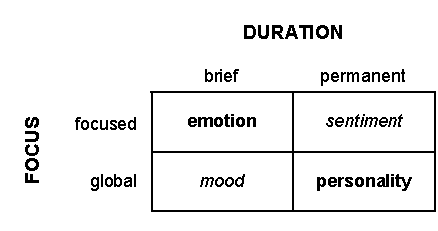
\includegraphics[width=0.45\textwidth]{figures/CR_affectTypes.pdf}

                \caption[Proposed Relation Between Emotion and Other Affective
                Types]{Proposed Relation Between Emotion and Other Affective
                Types (Adapted from \citet[p.~136]{moffat1997personality})}
                \label{fig:CRAffectTypes}
            \end{figure}

            \item Could derive core affect from emotion process via the
            \textit{valence} and \textit{demand character} appraisal
            dimensions and arousal value~\citep[p.~207,
            454]{frijda1986emotions}
        \end{itemize}

        \item Inclusion of a ``Regulation Processes" block that can affect
        nearly all parts of the emotion
        process~\citep[p.~545]{frijda1986emotions}
        \begin{itemize}
            \item Multiple points to introduce new components and processes
            $\rightarrow$ easy to add non-affective components

            \item Potential to violate \textit{Hiding the Complexity of Emotion
                Generation} (\ref{easeHide}) if users can access points directly
            $\rightarrow$ create an interface to hide entry points, make it
            easier to use and understand
        \end{itemize}
    \end{itemize}

    \item \textbf{Lazarus} (\weak)
    \begin{itemize}
        \item Personality not seen as a set of innate traits that manifest in
        appraisal and coping~\citep[p.~316]{lazarus1991emotion}, defined as a
        collection of goals, needs, commitments, knowledge, attitudes, and
        beliefs that influence how an event is perceived and how the individual
        acts on the resulting action tendency~\citep[p.~623--624,
        628]{smith1990emotion} $\rightarrow$ implicitly defined
        \begin{itemize}
            \item  Affords flexibility (i.e. not limited to a set of values)
            $\rightarrow$ supports creative freedom, definitions of individual
            characters based on their goals and knowledge rather than numerical
            values

            \item More difficult to define personality quickly (e.g. have to
            decide what beliefs a character with a desired personality would
            have)
        \end{itemize}

        \item Mood is ``an existential state or condition of life'' that is
        appraisal-dependent, related to subjective
        well-being~\citep[p.~266--267]{lazarus1991emotion}
        \begin{itemize}
            \item Could define as a state that aggregates appraisal results
            into a ``satisfaction/dissatisfaction'' value
        \end{itemize}

        \item Equates affect to subjective
        experience~\citep[p.~57]{lazarus1991emotion}
        \begin{itemize}
            \item Could define core affect using \textit{goal congruence} as
            \textit{valence}

            \item arousal is part of an action tendency, tied to the
            emotion's core relational theme~\citep[p.~58--59,
            150]{lazarus1991emotion} $\rightarrow$ not explicitly defined
        \end{itemize}

        \item Potential interface points for external processes part of input
        generation/output manipulation~\citep[p.~210]{lazarus1991emotion}
        $\rightarrow$ does not have to integrate with emotion generation
        process, trivial to add non-affective components
    \end{itemize}

    \item \textbf{Scherer} (\weak)
    \begin{itemize}
        \item Proposes definitions for mood and
        personality~\citep[p.~140--141]{scherer2000psychological}, but are not
        accounted for in the working theory~\citep[p.~93,
        119]{scherer2001appraisalB}
        \begin{itemize}
            \item Personality could be defined as sensitivities in appraisal
            dimension and register functions, mood as temporary sensitivities
            caused by previous appraisals $\rightarrow$ potential to violate
            psychological validity
        \end{itemize}

        \item No clear connection to core affect

        \item Potential to integrate non-affective components at the
        information processing, appraisal objective
        steps~\citep[p.~104]{scherer2001appraisalB} $\rightarrow$ might require
        knowledge of how those components work, violating \textit{Hiding the
            Complexity of Emotion Generation} (\ref{easeHide})
    \end{itemize}

    \item \textbf{Roseman} (\weak)
    \begin{itemize}
        \item Suggests that mood and personality are tied to emotion
        generation~\citep[p.~81--83]{roseman2001model}, ways to describe
        appraisal styles for individual or families of
        emotion~\citep[p.~88--89]{roseman2001model} $\rightarrow$ implicitly
        defined
        \begin{itemize}
            \item  Affords flexibility (i.e. not limited to a set of values)
            $\rightarrow$ supports creative freedom, definitions of individual
            characters based on their goals and knowledge rather than numerical
            values

            \item More difficult to define quickly (e.g. have to decide what
            appraisal dispositions a character with a desired personality would
            have)

            \item Could be extended to represent cultural influences on emotion
            generation
        \end{itemize}

        \item No clear connection to core affect
        \begin{itemize}
            \item Could define core affect using \textit{situational state} and
            \textit{motivational state} as \textit{valence}

            \item No obvious component for arousal
        \end{itemize}

        \item Focus on the relationship between appraisal values and
        emotions~\citep[p.~81]{roseman2001model} $\rightarrow$ does not focus
        on other parts of the generation process, no obvious place to integrate
        non-affective processes
    \end{itemize}

    \item \textbf{OCC} (\strong)
    \begin{itemize}
        \item Proposes that personality is a unique parameter profile defining
        how emotion generation behaves within and between process
        levels~\citep[p.~189--190]{ortony2005affect}
        \begin{itemize}
            \item Tuning emotion generation for each NPC $\rightarrow$
            personality implicitly supported by \textit{Customizing Existing
                CME Task Parameters} (\ref{flexCustom})

            \item Could implement personality inventories as parameter
            profiles~\citep[p.~191--192]{ortony2005affect} $\rightarrow$ no
            explicit definitions given, potential to violate psychological
            validity if done incorrectly, might not matter if the profiles do
            what the developer expects
        \end{itemize}

        \item Moods described as free-floating, object-less affective states
        that can influence emotion but can also arise from sources
        independently of emotion~\citep[p.~27]{clore2000cognition}
        $\rightarrow$ could be linked to personality ``parameter profiles'' by
        treating it as an initial condition
        \begin{itemize}
            \item Defined as temporally-driven parameter changes~\citep[p.~184,
            189--190]{occ} $\rightarrow$ implicitly supported by
            \textit{Customizing Existing CME Task Parameters} (\ref{flexCustom})
        \end{itemize}

        \item Potential to represent core affect
        \begin{itemize}
            \item Physiological arousal is a global intensity variable,
            roughly proportional to base emotion
            intensity---approximately represented by the sum of the absolute
            unsigned values of some variables\footnote{\textit{desireability},
                \textit{undesireability}, \textit{praiseworthiness},
                \textit{blameworthiness}, \textit{appealingness}, and
                \textit{unappealingness}}---or perhaps even only parts of this
            (i.e. subjective importance of the situation)~\citep[p.~51,
            65--66]{occ} $\rightarrow$ other factors can influence it, and has
            a slow rate of decay, supports \textit{Customizing Existing CME
                Task Parameters} (\ref{flexCustom})

            \item It follows that \textit{valence} might be approximated as sum
            of the absolute signed values of the same variables (i.e. is the
            overall feeling positive or negative?)
        \end{itemize}

        \item Two potential ways to integrate non-affective components
        \begin{itemize}
            \item As part of the input generation process $\rightarrow$
            designer-driven, supports \textit{Ability to Operate on Different
                Levels of NPC Complexity} (\ref{flexComplex})

            \item As a method for controlling task parameters $\rightarrow$
            implicitly supported by \textit{Customizing Existing CME Task
                Parameters} (\ref{flexCustom})
        \end{itemize}
    \end{itemize}

    \item \textbf{Smith \& Kirby} (\weak)
    \begin{itemize}
        \item No clear definitions for personality, mood, or core affect
        \begin{itemize}
            \item Potential correlation between \textit{emotion-focused coping
                potential} and some personality traits~\citep[p.~1366--1368,
            1369]{smith2009putting} $\rightarrow$ suggests that personality are
            parameters on the emotion generation process

            \item Core affect could be constructed from \textit{motivational
                congruence} (as \textit{valence}) and \textit{motivational
                relevance}
            (as arousal) $\rightarrow$ not necessarily empirically
            supported, potential to violate psychological validity
        \end{itemize}

        \item Appraisal registers synthesize information from multiple sources,
        levels of processing~\citep[p.~130]{smith2001toward}
        \begin{itemize}
            \item Multiple points to introduce new components and processes
            $\rightarrow$ easy to add non-affective components

            \item Integrating non-affective components would require
            manipulating the detector mechanisms, potential to violate
            \textit{Hiding the Complexity of Emotion Generation}
            (\ref{easeHide}) if users can access points directly $\rightarrow$
            create an interface to hide entry points, make it easier to use and
            understand
        \end{itemize}
    \end{itemize}

    \item \textbf{Oatley \& Johnson-Laird} (\strong)
    \begin{itemize}
        \item Emotions often have moods and sentiments associated with
        them~\citep[p.~87]{oatley2000sentiments} $\rightarrow$ implies that
        adding these affective types would be an extension of existing emotion
        structures

        \item Temperaments (i.e. personality traits) hypothesized to be enduring
        predispositions towards emotion ``modes''
        (\citepg{oatley1987towards}{34}; \citepg{oatley1992best}{61})
        \begin{itemize}
            \item Also defines sentiments---enduring emotional dispositions
            about something, typically other
            individuals~\citep[p.~81]{oatley2000sentiments} $\rightarrow$
            potential to define two sets of personality traits (general and
            target-specific), affords more creative freedom
        \end{itemize}

        \item Moods defined directly in the theory as control signals that
        persist after the cause of an emotion passes/no longer associated with
        semantic content and keeps the system in a particular state
        (\citepg{oatley1987towards}{32}; \citepg{oatley1992best}{64})
        \begin{itemize}
            \item Could be realized as a temporary predispositions towards
            emotion ``modes'' or a longer lasing, low intensity emotion
            state~\citep[p.~34--35]{oatley1987towards} $\rightarrow$ potential
            to allow both, give user the choice of which to use, affording more
            creative freedom
        \end{itemize}

        \item Potential to define core affect based on how a goal is affected
        (positive or negative) for \textit{valence}, emotion intensity as
        arousal $\rightarrow$ no explicit definitions given, potential to
        violate psychological validity if done incorrectly, might not matter if
        the profiles do what the developer expects

        \item Assume that the cognitive system is modular and
        asynchronous~\citep[p.~31]{oatley1987towards} $\rightarrow$ implies
        that adding non-affective processes is feasible, should not require
        knowledge of the inner workings of emotion generation
    \end{itemize}
\end{itemize}

\subsubsection{Flexibility: Choosing NPC Emotions (\ref{flexEm})}
Like the discrete theories, the appraisal theories tend to define emotions as
categories to group different aspects of a response together. In this sense,
excluding predefined emotions is trivial. Once again, \textit{adding} new ones
is unclear and there are no obvious ``rules'' to follow. \progname{} can still
take advantage of them though, because new emotions need only make sense to the
developer so that they can use them. Therefore, the appraisal theories are
evaluated for what a developer would need to do and how easy it is to realize.

\begin{itemize}
    \item \textbf{Frijda} (\weak)
    \begin{itemize}
        \item Emotions as descriptions of action readiness in response to
        different combinations of events, or by the nature of the emotional
        object~\cite[p.~72--74]{frijda1986emotions} $\rightarrow$ defining new
        emotions requires defining new action tendencies
        \begin{itemize}
            \item Require modifications to the emotion generation process (i.e.
            defining appraisal patterns) $\rightarrow$ violates \textit{Hiding
                the Complexity of Emotion Generation} (\ref{easeHide})

            \item Some ``non-basic'' emotions are blends, can define a limited
            set of additional emotions $\rightarrow$ limited flexibility

            \item Define emotions by pairing existing ones with an event or
            object type and assigning it a new name $\rightarrow$ similar to
            scripting, event-coding
        \end{itemize}
    \end{itemize}

    \item \textbf{Lazarus} (\weak)
    \begin{itemize}
        \item Emotions associated with themes that can
        coexist~\citep[p.~229]{lazarus1991emotion}
        \begin{itemize}
            \item Potential to allow developers to create named combinations
            representing ``new'' emotions $\rightarrow$ necessarily create more
            complicated emotions

            \item Defining emotions that are not combinations would require new
            appraisal pattern definitions (i.e. modify emotion generation
            process) $\rightarrow$ violates \textit{Hiding the Complexity of
                Emotion Generation} (\ref{easeHide})
        \end{itemize}
    \end{itemize}

    \item \textbf{Scherer} (\good)
    \begin{itemize}
        \item ``Emotions'' defined as the net effect of continuous,
        fluctuating subsystem changes~\citep[p.~106, 108]{scherer2001appraisalB}
        \begin{itemize}
            \item Adding new emotions requires identification and naming of a
            set of subsystem changes (i.e. requires an understanding of how
            emotions are generated) $\rightarrow$ violates \textit{Hiding the
                Complexity of Emotion Generation} (\ref{easeHide})
        \end{itemize}

        \item ``Innate'' emotions\footnote{Scherer calls them \textit{modal}
            emotions.} (e.g. \textit{Joy}) attributed to common adaptational
            issues
        that produce consistent system effects~\citep[p.~108,
        113]{scherer2001appraisalB} $\rightarrow$ range of known emotions are
        products of mixtures and/or blends of ``innate'' ones
        \begin{itemize}
            \item Some emotion profiles have ``open'' entries that can accept
            any value for that dimension $\rightarrow$ potential to define
            emotion family ``members'' by providing specific values for
            ``open'' entries, potential to violate \textit{Hiding the
                Complexity of Emotion Generation} (\ref{easeHide})

            \item Intensity differences can also differentiate otherwise
            identical emotions $\rightarrow$ define new emotions by intensity
            class, external to the emotion generation process so no violation
            of \textit{Hiding the Complexity of Emotion Generation}
            (\ref{easeHide})
        \end{itemize}
    \end{itemize}

    \item \textbf{Roseman} (\good)
    \begin{itemize}
        \item Proposes that more than one emotion can be experienced
        simultaneously due to different
        evaluations~\citep[p.~81]{roseman2001model}
        \begin{itemize}
            \item Definition of new emotions as mixtures $\rightarrow$ external
            to the generation process, so no violation of \textit{Hiding the
                Complexity of Emotion Generation} (\ref{easeHide})

            \item Emotions are logically grouped by response strategy (e.g.
            \textit{attack}, \textit{exclude}) $\rightarrow$ potential for a
            design tool to guide the process of defining new emotions?
        \end{itemize}
    \end{itemize}

    \item \textbf{OCC} (\good)
    \begin{itemize}
        \item Emotions necessarily tied to cognitive abilities that build on
        four basic affective states~\citep[p.~183--184]{ortony2005affect}
        implies that adding ``new'' emotions is about adding meaning
        $\rightarrow$ dependent on what is available for inputs,
        designer-driven, supports \textit{Ability to Operate on Different
            Levels of NPC Complexity} (\ref{flexComplex})

        \item Propose smaller emotion structure for believable agents,
        collapsing 22 emotions into five positive and five negative
        ones~\citep[p.~193--194]{ortony2002making}
        \begin{itemize}
            \item Potential to add ``new'' emotions as more cognitive processes
            are added $\rightarrow$ dependent on what is available for inputs,
            designer-driven, supports \textit{Ability to Operate on Different
                Levels of NPC Complexity} (\ref{flexComplex})
        \end{itemize}

        \item \textit{Surprise} as a special case, can be added in connection
        with the \textit{unexpectedness} appraisal variable~\citep[p.~13--14,
        16--17]{ortony2021all}

        \item ``New'' emotions can be defined as differences in
        intensity/elicitation thresholds (e.g. \textit{Pleased} for low
        intensity and \textit{Ecstatic} for high)~\citep[p.~185]{occ}
        \begin{itemize}
            \item External to the emotion generation process $\rightarrow$ no
            violation of \textit{Hiding the Complexity of Emotion Generation}
            (\ref{easeHide})
        \end{itemize}
    \end{itemize}

    \item \textbf{Smith \& Kirby} (\weak)
    \begin{itemize}
        \item Unclear how additional emotions could be defined

        \item Hypothesizes that emotion categories are likely dense clusters in
        dimensional space~\citep[p.~245--246]{smith_scott_mandler_1997}
        \begin{itemize}
            \item Potential to combine with V-A or PAD Space, define new
            emotion categories from existing data clusters $\rightarrow$ would
            require some understanding of source material, potential violation
            of \textit{Hiding the Complexity of Emotion Generation}
            (\ref{easeHide})

            \item Developers could collect their own data to find affective
            ``clusters'' in a dimensional space $\rightarrow$ time consuming,
            error-prone, potential violation of \textit{Hiding the Complexity
                of Emotion Generation} (\ref{easeHide})
        \end{itemize}
    \end{itemize}

    \item \textbf{Oatley \& Johnson-Laird} (\strong)
    \begin{itemize}
        \item How people describe emotions in everyday language indicates
        underlying cognitive meanings~\citep[p.~210]{johnson1992basic}
        $\rightarrow$ can build on layperson's understanding of emotions,
        supports \textit{Hiding the Complexity of Emotion Generation}
        (\ref{easeHide})

        \item Emotion ``modes'' are not absolute definitions, only have
        heuristic properties that capture general classes of
        events~\citep[p.~87]{oatley2000sentiments} $\rightarrow$ potential to
        create more refined emotions by constraining the classes
        \begin{itemize}
            \item ``New''/''adult'' emotions are based on emotion ``modes'',
            deliberative processes attach more meaning to them
            (\citepg{oatley1987towards}{35, 43};
            \citepg{oatley1992best}{76--78})

            \item Can also be defined at junctions of mutual plans with one or
            more other agents, requires a self-model~\citep[p.~44, 46,
            48]{oatley1987towards} $\rightarrow$ way to integrate cultural
            differences due to the impact on models and reasoning
            processes~\citep[p.~47]{oatley1987towards}
        \end{itemize}

        \item Emotions that have different semantic contents can exist
        simultaneously~\citep[p.~104]{oatley1992best} $\rightarrow$ potential
        to define emotion ``mixtures''
        \begin{itemize}
            \item External to the emotion generation process $\rightarrow$ no
            violation of \textit{Hiding the Complexity of Emotion Generation}
            (\ref{easeHide})
        \end{itemize}
    \end{itemize}
\end{itemize}

\subsubsection{Flexibility: Allowing Developers to Specify How to Use CME
Outputs
    (\ref{flexOut})}
There is clearly a difference between reflexes and emotions: one is very
difficult to control how one reacts and the other has a range of them to pick
from~\citep[p.~45]{fellous2004human}. The idea of emotion \textit{components}
also suggests that there is flexibility in which system aspects are affected
and how (\citepg{hudlicka2019modeling}{133};
\citepg{scherer2001appraisalB}{108}; \citepg{roseman2011emotional}{436}). This
implies that \textit{any} appraisal theory should be able to strongly support
this requirement. The question is now how well each theory defines what this
means.

\begin{itemize}
    \item \textbf{Frijda} (\strong)
    \begin{itemize}
        \item Set the output boundary of \progname{} at the action proposer
        (i.e. action tendency), relevance and control precedence signals, and
        physiological change generators (i.e. arousal)
        points~\citep[p.~455]{frijda1986emotions}
        \begin{itemize}
            \item Would also allow for another layer to group these into
            emotion categories~\citep[p.~72]{frijda1986emotions}

            \item Can feed the outputs back into \progname{} $\rightarrow$
            provide an interface so that this is a matter of ``flipping a
            switch'', supported by \textit{Customizing Existing CME Task
                Parameters} (\ref{flexCustom})

            \item [$\rightarrow$] Allows maximum flexibility for defining what
            to do with outputs that is agnostic to how ``action'' is defined
        \end{itemize}
    \end{itemize}

    \item \textbf{Lazarus} (\strong)
    \begin{itemize}
        \item Set the output boundary of \progname{} at the appraisal outcome
        (i.e. action tendency, subjective experience, physiological response),
        would also allow for labelling the output with emotion
        categories~\citep[p.~209--210]{lazarus1991emotion}
        \begin{itemize}
            \item Excludes coping process integral to the theory $\rightarrow$
            could be added as an external component, supported by
            \textit{Allowing the Integration of New CME Components}
            (\ref{flexNew})

            \item Resulting NPC actions would impact their interpretation of
            the environment $\rightarrow$ implicitly supports reappraisal
            process~\citep[p.~134]{lazarus1991emotion}

            \item Can feed the outputs back into \progname{} $\rightarrow$
            provide an interface so that this is a matter of ``flipping a
            switch'', supported by \textit{Customizing Existing CME Task
                Parameters} (\ref{flexCustom})

            \item [$\rightarrow$] Allows maximum flexibility for defining what
            to do with outputs that is agnostic to how ``action'' is defined
        \end{itemize}
    \end{itemize}

    \item \textbf{Scherer} (\strong)
    \begin{itemize}
        \item Set the output boundary of \progname{} at the action tendency
        level, would also allow for labelling the output with emotion
        categories~\citep[p.~107, 113]{scherer2001appraisalB} $\rightarrow$
        allows maximum flexibility for defining what to do with outputs that is
        agnostic to how ``action'' is defined

        \item Allow users to access individual appraisal
        registers~\citep[p.~104]{scherer2001appraisalB} $\rightarrow$ affords
        more flexibility
        \begin{itemize}
            \item Each part of the appraisal process makes changes to different
            subsystems, creates a continuously changing
            outputs~\citep[p.~107]{scherer2001appraisalB} $\rightarrow$
            appraisal ``history" encoded in unique pattern caused by subsystem
            changes, values update frequently

            \item Potential to violate \textit{Hiding the Complexity of Emotion
                Generation} (\ref{easeHide}) $\rightarrow$ make available for
            advanced users

            \item Potential to violate psychological validity $\rightarrow$ how
            a user uses the values should be external to \progname{}, so its
            internal psychological validity would remain intact
        \end{itemize}
    \end{itemize}

    \item \textbf{Roseman} (\strong)
    \begin{itemize}
        \item Set the output boundary of \progname{} at the ``response
        strategy'', the typical physiological, phenomenological, expressive,
        behavioural, and motivational emotion contents
        (\citepg{roseman2013appraisal}{141}; \citepg{roseman2001model}{75};
        \citepg{roseman2018functions}{146--148, 151--152})
        \begin{itemize}
            \item Potential to connect components directly to existing game
            modules if available (e.g. ``expressive'' as an input to NPC
            animation, ``motivation'' to planning) $\rightarrow$ user chooses
            which ones to use, supported by \textit{Choosing Which CME Tasks to
                Use} (\ref{flexTasks})

            \item Differentiates between ``action tendency'' and what action is
            actually taken, informed by emotion
            intensity~\citep[p.~436]{roseman2011emotional} $\rightarrow$ input
            to the behaviour/expression selection process, explicitly built-in
            support for \textit{Allowing Developers to Specify How to Use CME
                Outputs} (\ref{flexOut})

            \item Also notes that there is consistency in what types of
            responses that each emotion elicits~\citep{roseman2011emotional}
            $\rightarrow$ creates consistent behaviour necessary for
            believability~\citep[p.~200]{ortony2002making}

            \item [$\rightarrow$] Allows maximum flexibility for defining what
            to do with outputs that is agnostic to the system at large
        \end{itemize}
    \end{itemize}

    \item \textbf{OCC} (\strong)
    \begin{itemize}
        \item Set the output boundary of \progname{} at the evaluation of
        emotion category and intensity~\citep[p.~19, 69]{occ}
        \begin{itemize}
            \item Propose that action tendencies are not necessary or
            sufficient to define emotion because some emotions might not have a
            ``characteristic" action tendency as defined as voluntary actions
            following emotion~\citep[p.~11]{occ} $\rightarrow$ allows the
            generation of emotions that do not have one, removes constraint
            from user

            \item Claims ``action tendency'' is a set of components that
            emotions constrain themselves to, but might not use all
            components~\citep[p.~198, 201]{ortony2002making} $\rightarrow$
            creates consistent behaviour necessary for
            believability~\citep[p.~200]{ortony2002making}

            \item [$\rightarrow$] Allows maximum flexibility for defining what
            to do with outputs that is agnostic to the system at large
        \end{itemize}
    \end{itemize}

    \item \textbf{Smith \& Kirby} (\strong)
    \begin{itemize}
        \item Set the output boundary of \progname{} at ``emotional response'',
        contains appraisal outcome (e.g. emotion category and dimensions,
        intensity), physiological activity (e.g. arousal, facial
        expressions), and action tendencies~\citep[p.~123, 130]{smith2001toward}
        \begin{itemize}
            \item Users can separate components and send them to different
            system process

            \item Can also send components back into appraisal processes via
            appraisal sources $\rightarrow$ potential for different
            interpretations due to processing in appraisal
            source~\citep[p.~99]{smith2000consequences}

            \item [$\rightarrow$] Allows maximum flexibility for defining what
            to do with outputs that is agnostic to the system at large
        \end{itemize}
    \end{itemize}

    \item \textbf{Oatley \& Johnson-Laird} (\strong)
    \begin{itemize}
        \item Set the output boundary of \progname{} at control signals,
        labelled with an emotion category~\citep[p.~50, 54]{oatley1992best}

        \item Control signals are global entities or ``alarms'' that change the
        system ``mode'' when a goal is impacted by an active plan, bringing it
        into focus~\citep[p.~62--63]{oatley1992best}
        \begin{itemize}
            \item Users can choose which system components are receptive to the
            signal and to what degree $\rightarrow$ supported by
            \textit{Choosing Which CME Tasks to Use} (\ref{flexTasks}) and
            \textit{Customizing Existing CME Task Parameters} (\ref{flexCustom})

            \item [$\rightarrow$] Allows maximum flexibility for defining what
            to do with outputs that is agnostic to the system at large
        \end{itemize}
    \end{itemize}
\end{itemize}

\subsubsection{Flexibility: Ability to Operate on Different Levels of NPC
    Complexity (\ref{flexComplex})}
Due to the assumed role of cognition in emotion processes
(\citepg{marsella2015appraisal}{55}; \citepg{broekens2021emotion}{354}), there
is also an assumed level of NPC complexity needed for an appraisal-based CME to
properly function. Therefore, the appraisal theories are evaluated based on how
much cognitive processing is required to produce results.

\begin{itemize}
    \item \textbf{Frijda} (\weak)
    \begin{itemize}
        \item Requires encoded categories for events and rules for inputs,
        action structures for evaluating coping, process to evaluate
        event/action implications, definition of concern
        structures~\citep[p.~457]{frijda1986emotions} $\rightarrow$ effort to
        create likely to linearly increase with respect to game complexity
        \begin{itemize}
            \item Some can be implicitly evaluated in \progname{} $\rightarrow$
            relieves some of the authorial burden from game designers
        \end{itemize}

        \item Regulation processes can be added as needed, not mandated in the
        core emotion process~\citep[p.~454, 456]{frijda1986emotions}
        $\rightarrow$ can potentially adapt to increases in NPC/game complexity
        \begin{itemize}
            \item Path in process to add planning if needed, but not critical to
            function~\citep[p.~462]{frijda1986emotions}
        \end{itemize}

        \item Requires a monitoring process (i.e. blackboard structure) to
        continuously update situational
        meaning~\citep[p.~459]{frijda1986emotions} $\rightarrow$ space
        requirements increases with information sources

    \end{itemize}

    \item \textbf{Lazarus} (\strong)
    \begin{itemize}
        \item Purpose of appraisal is to ``integrate the two [personal
        interests with environmental realities] as effectively as
        possible''~\citep[p.~135]{lazarus1991emotion} $\rightarrow$ complexity
        controlled by \progname{}, can be made relatively simple

        \item Complexity in individual factors and environmental conditions
        evaluations that get passed to
        appraisal~\citep[p.~209--210]{lazarus1991emotion} $\rightarrow$
        designer controlled, can define to match game complexity
        \begin{itemize}
            \item Minimally requires definitions for goals, ``ego type", event
            causes, predictions about the impact of actions and future
            events~\citep[p.~149--150]{lazarus1991emotion}

            \item [$\rightarrow$] Could connect to hard-coded data/processes
            for low-complexity games (e.g. \textit{Pac-Man}~\citep{pacman}),
            increase complexity with game
        \end{itemize}

        \item Implication of a central data structure to store appraisal values
        as they become available~\citep[p.~134, 151, 189,
        210--211]{lazarus1991emotion}
        \begin{itemize}
            \item Stores outputs of appraisal evaluations, not the inputs

            \item [$\rightarrow$] Complexity likely to be constant or linearly
            increase with respect to the number and complexity of inputs
        \end{itemize}
    \end{itemize}

    \item \textbf{Scherer} (\strong)
    \begin{itemize}
        \item Built-in support for variable NPC complexity
        \begin{itemize}
            \item Appraisal dimension groupings (SECs) can be as complex as the
            information processing system allows, often a continuous or graded
            scalar or multidimensional
            evaluation~\citep[p.~94]{scherer2001appraisalB} $\rightarrow$
            numerical values easier to manipulate

            \item Assumes three levels of processing (sensory-motor, schematic,
            conceptual) that
            interact~\citep[p.~102--103]{scherer2001appraisalB} $\rightarrow$
            potential to derive some information in \progname{} implicitly from
            inputs
            \begin{itemize}
                \item Provide option to turn these tasks off or configure them
                $\rightarrow$ support for \textit{Choosing Which CME Tasks to
                    Use} (\ref{flexTasks}) and \textit{Customizing Existing
                    Task
                    Parameters} (\ref{flexCustom})
            \end{itemize}
        \end{itemize}

        \item Reappraisals run until a monitoring system signals termination or
        adjustment, appraisal components updated by
        reappraisals~\citep[p.~99]{scherer2001appraisalB} $\rightarrow$ game
        designer can decide when to terminate appraisal cycles based on game
        needs, support of \textit{Customizing Existing Task Parameters}
        (\ref{flexCustom}) and \textit{Be Efficient and Scalable}
        (\ref{flexScale})

        \item Appraisal registers updated as new information becomes available,
        central structure, can control relative importance of each
        value using a weighted function to represent ``goodness'' of
        data~\citep[p.~105]{scherer2001appraisalB};
        \begin{itemize}
            \item Implies a temporal and confidence value for each
            register~\citep[p.~106]{scherer2001appraisalB} $\rightarrow$ game
            designer can decide when to evaluate emotion state based on these
            values, support of \textit{Customizing Existing Task Parameters}
            (\ref{flexCustom})
        \end{itemize}
    \end{itemize}

    \item \textbf{Roseman} (\good)
    \begin{itemize}
        \item Suggestion that there are different versions of appraisal
        mechanisms of variable complexity triggered as time
        allows~\citep[p.~77]{roseman2001model}, and influenced by emotion
        intensity~\citep[p.~440]{roseman2011emotional}
        \begin{itemize}
            \item Can specify different appraisal mechanisms $\rightarrow$ game
            designers can build on top of input API, choose how information is
            synthesised into \progname{} inputs
        \end{itemize}

        \item Still requires empirical data to determine the minimum cognitive
        requirements for appraisals~\citep[p.~87--88]{roseman2001model}
        \begin{itemize}
            \item Lowest level involves fixed action
            patterns~\citep[p.~32]{clore2000cognition} $\rightarrow$
            correspondence with core \progname{} tasks, direct match between
            generated emotion and assigned behaviours for it as assigned by
            game designer

            \item With no defined process, do not know how to integrate
            cognitive processes into \progname{}
        \end{itemize}
    \end{itemize}

    \item \textbf{OCC} (\good)
    \begin{itemize}
        \item Has three levels of processing (reactive, routine,
        reflective)~\citep[p.~175--177, 179]{ortony2005affect}
        \begin{itemize}
            \item OCC proper part of the highest processing level,
            ``reflective'', does not interact with external environment
            $\rightarrow$ requires cognitive/high-level
            processes, inputs from other two levels

            \item Number of potential emotions restricted in reactive (no
            emotions) and routine (four emotions) levels $\rightarrow$ violates
            \textit{Choosing NPC Emotions} (\ref{flexEm})

            \item Assumptions make it unlikely to be applicable to
            architectures that are simpler than adult
            humans~\citep[p.~220]{sloman2005architectural}
        \end{itemize}

        \item Produce a simpler, less rigorous architecture with one processing
        level
        \begin{itemize}
            \item Complexity might lie in how variables are evaluated and how
            goals/standards/attitudes are represented, coding of rules appears
            relatively simple~\citep[p.~182--188]{occ}

            \item Could allow for user-defined evaluations and representations
            $\rightarrow$ support as a Domain-Specific Language (DSL) to avoid
            violating \textit{Hiding the Complexity of Emotion Generation}
            (\ref{easeHide})
        \end{itemize}
    \end{itemize}

    \item \textbf{Smith \& Kirby} (\strong)
    \begin{itemize}
        \item Potential to design multiple appraisal mechanisms that rely
        on different functions (e.g. planning, expectation evaluation)
        $\rightarrow$ clear distinction between available functions and
        \progname{}'s abilities
        \begin{itemize}
            \item Number of appraisal variables determines types of emotion
            available~\citep{yih2016distinct, yih2016patterns},
            \citep[p.~488--492]{yih2020profiles}

            \item [$\rightarrow$] Number of potential emotion categories tied
            to NPC complexity

            \item Potential to violate \textit{Choosing NPC Emotions}
            (\ref{flexEm}) $\rightarrow$ assuming that NPC complexity and what
            emotions the game designer wants them to have are directly
            proportional, this is unlikely to be a concern
        \end{itemize}
    \end{itemize}

    \item \textbf{Oatley \& Johnson-Laird} (\good)
    \begin{itemize}
        \item Distinguishing emotion types changes based on cognitive
        abilities~\citep[p.~40--41]{oatley1987towards}, possible goal and plan
        representations~\citep[p.~57--58]{oatley1992best}
        \begin{itemize}
            \item Emotion ``modes'' as ``base classes'' of emotion

            \item [$\rightarrow$] Number of potential emotion categories tied
            to NPC complexity

            \item Potential to violate \textit{Choosing NPC Emotions}
            (\ref{flexEm}) $\rightarrow$ assuming that NPC complexity and what
            emotions the game designer wants them to have are directly
            proportional, this is unlikely to be a concern
        \end{itemize}
    \end{itemize}
\end{itemize}

\subsubsection{Flexibility: Be Efficient and Scalable (\ref{flexScale})}
The main concern for the efficiency and scalability of the appraisal theories
is how they evaluate inputs. However, this complexity seems to lie in creating
the inputs. Since this precedes their transformation into emotions, action
tendencies, and other components, a lot of this burden is passed to the game
developer. Ideally, \progname{} would handle more of these tasks. However, this
also allows developers to choose how they want to generate inputs. Ultimately
this gives them more freedom, and allows \progname{} to merge more easily into
different games and underlying architectures. What \progname{} focuses on,
then, is helping game developers manage different evaluation processes.

\begin{itemize}
    \item \textbf{Frijda} (\good)
    \begin{itemize}
        \item Uses 17--24 appraisal dimensions to create unique profiles for
        emotions, not all dimensions needed for each emotion
        (\citepg{frijda1986emotions}{205--219};
        \citepg{frijda1987emotion}{121--124})
        \begin{itemize}
            \item Efficiency might be hindered if more dimensions are evaluated
            than are needed

            \item Give developers choice of appraisal dimensions $\rightarrow$
            compromises \textit{Hiding the Complexity of Emotion Generation}
            (\ref{easeHide})
        \end{itemize}

        \item Scalability mostly driven by complexity of inputs and
        externally-defined regulation processes $\rightarrow$ depends on
        complexity of evaluations to generate inputs, designer-driven
    \end{itemize}

    \item \textbf{Lazarus} (\strong)
    \begin{itemize}
        \item Dependent on knowledge~\citep[p.~145]{lazarus1991emotion},
        knowledge evaluation mechanisms $\rightarrow$ depends on designer chosen
        architecture

        \item Appraisal process appears to be of a fixed complexity once inputs
        are given~\citep[p.~210]{lazarus1991emotion}, implies that scalability
        depends on complexity of knowledge processes and inputs $\rightarrow$
        depends on complexity of evaluations to generate inputs, designer-driven
    \end{itemize}

    \item \textbf{Scherer} (\good)
    \begin{itemize}
        \item Uses 16 appraisal dimensions divided into four
        groups~\citep[p.~114--115]{scherer2001appraisalB} $\rightarrow$ minimum
        set of appraisal dimensions necessary to differentiate emotion
        families~\citep[p.~94]{scherer2001appraisalB}

        \item Groups are evaluated in order to avoid using unneeded expensive
        processes~\citep[p.~99--100, 102--103]{scherer2001appraisalB}
        \begin{itemize}
            \item Does not exclude potential to begin getting partial results by
            running the four components in parallel

            \item Groups can have more than one associated process
            $\rightarrow$ lower level processes for each group first, higher
            level processes only used if they do not return results

            \item Can add a central controller to allow integration of
            additional processes similar to Smith \& Kirby appraisal
            detector~\citep[p.~103--105]{scherer2001appraisalB}

            \item [$\rightarrow$] Efficiency tied to the complexity of inputs,
            partially designer-driven

            \item [$\rightarrow$] Mechanisms for scalability built-in, but
            requires more overhead costs to manage them, might conflict with
            \textit{Ability to Operate on Different Levels of NPC Complexity}
            (\ref{flexComplex})
        \end{itemize}
    \end{itemize}

    \item \textbf{Roseman} (\weak)
    \begin{itemize}
        \item Suggests that there are different versions of appraisal
        mechanisms of variable complexity triggered as time
        allows~\citep[p.~77]{roseman2001model} $\rightarrow$ potential for
        scalability, efficiency

        \item Focuses on the structure of emotions and appraisal
        dimensions~\citep[p.~68, 81]{roseman2001model} $\rightarrow$ no further
        information given
    \end{itemize}

    \item \textbf{OCC} (\good)
    \begin{itemize}
        \item Uses 3--19 variables to differentiate emotion families, not all
        variables needed for each emotion~\citep[p.~19, 60, 69]{occ}
        $\rightarrow$ can prevent evaluation of some variables based on which
        branch of the tree is active

        \item Efficiency tied to complexity of inputs~\citep[p.~182--188]{occ}
        $\rightarrow$ tied to evaluation mechanisms, designer-driven

        \item Can introduce mechanisms such that lower-complexity processes run
        first and call higher-complexity processes if they cannot produce a
        result~\citep[p.~179]{ortony2005affect} $\rightarrow$ more control of
        efficiency and scalability

        \item Can have two parallel emotion-elicitation mechanisms
        $\rightarrow$ can produce conflicting results~\citep[p.~37--39,
        54]{clore2000cognition}
        \begin{itemize}
            \item Memory-based heuristics, which is faster and more error-prone
            $\rightarrow$ improved efficiency, could run into memory-related
            scalability issues

            \item Deliberative processing, which is slower and less error-prone
            $\rightarrow$ reduced efficiency, more scale-friendly

            \item [$\rightarrow$] Could create a more believable result, but
            might conflict with \textit{Ability to Operate on Different Levels
                of NPC Complexity} (\ref{flexComplex})
        \end{itemize}
    \end{itemize}

    \item \textbf{Smith \& Kirby} (\strong)
    \begin{itemize}
        \item Uses 7--16 variables to create unique profiles for emotions, not
        all dimensions needed for each emotion (\citepg{yih2020profiles}{489};
        \citeg{yih2016distinct})
        \begin{itemize}
            \item Efficiency might be hindered if more dimensions are evaluated
            than are needed

            \item Give developers choice of appraisal dimensions $\rightarrow$
            compromises \textit{Hiding the Complexity of Emotion Generation}
            (\ref{easeHide})
        \end{itemize}

        \item A few variables could be evaluated by \progname{} (e.g.
        \textit{motivational relevance}) $\rightarrow$ efficiency and
        scalability controlled by \progname{}

        \item Some evaluation processes produce inputs \textit{for} \progname{}
        $\rightarrow$ designer-driven, architecture dependent
        \begin{itemize}
            \item Appraisal detector continuously monitors for changes in
            variables, combines information and called appraisal
            process~\citep[p.~129--130]{smith2001toward} $\rightarrow$
            implicitly enforces scalability as developers add and remove
            processes
            \begin{itemize}
                \item Detector must only require minimal resources to function
                well~\citep[p.~90--91]{smith2000consequences} $\rightarrow$
                acknowledges that efficiency is essential
            \end{itemize}

            \item Support for multiple, parallel user-defined processes that
            could have variable complexity
            levels~\citep[p.~91--92]{smith2000consequences} $\rightarrow$
            create mechanism for developers to define when complex processes
            activate
        \end{itemize}
    \end{itemize}

    \item \textbf{Oatley \& Johnson-Laird} (\strong)
    \begin{itemize}
        \item Assumes a system that coordinates multiple plans and goals under
        time and resource constraints (e.g. plans only work 1--2 steps
        ahead)~\citep[p.~31, 36]{oatley1987towards} $\rightarrow$ property of
        the architecture, designer-driven

        \item Goals and plans associated with emotion has their own monitoring
        mechanisms~\citep[p.~50]{oatley1992best} $\rightarrow$ can decide which
        ones to associate with \progname{}, built in scalability
        \begin{itemize}
            \item Mechanism would work on goal and plan information
            $\rightarrow$ can be made efficient
        \end{itemize}

        \item Emotions can be given more complex meanings by evaluating more
        information via selective function
        calls~\citep[p.~32--34]{oatley1987towards} $\rightarrow$
        designer-dependent and ties scalability, efficiency to the needs of the
        game, supports \textit{Ability to Operate on Different Levels of NPC
            Complexity} (\ref{flexComplex})
    \end{itemize}
\end{itemize}

\subsubsection{Ease-of-Use: Hiding the Complexity of Emotion Generation
    (\ref{easeHide})}
The appraisal theories generally have strong support for this requirement.
Designers do not need to known what is done with the inputs they provide, so
the processing of those inputs can be hidden from them.

\begin{itemize}
    \item \textbf{Frijda} (\strong)
    \begin{itemize}
        \item System arranged so that information can be supplied at any point
        to black box processes, tracked by an internal monitor/situational
        meaning blackboard structure~\citep[p.~455--456,
        459]{frijda1986emotions} $\rightarrow$ do not need to know how the
        process uses information
    \end{itemize}

    \item \textbf{Lazarus} (\strong)
    \begin{itemize}
        \item Appraisal assigns personal meaning to
        knowledge~\citep[p.~145]{lazarus1991emotion} $\rightarrow$ do not need
        to know how the process uses information

        \item Six appraisal dimensions, reappraisal accounts for changes to
        input values~\citep[p.~134, 149--150]{lazarus1991emotion} $\rightarrow$
        can incorporate changing information as a queue of input values
    \end{itemize}

    \item \textbf{Scherer} (\strong)
    \begin{itemize}
        \item Inputs combined into
        registers~\citep[p.~105]{scherer2001appraisalB}, patterns of register
        values matched to emotions~\citep[p.~114--115]{scherer2001appraisalB}
        $\rightarrow$ do not need to know how this is done
        \begin{itemize}
            \item Some dimensions are pure information (e.g. \textit{intrinsic
                pleasantness})~\citep[p.~146]{lazarus1991emotion} $\rightarrow$
            inherently hides process complexity

            \item Appraisal dimension groupings (SECs) can be divided into
            hard-wired and deliberative
            units~\citep[p.~102]{scherer2001appraisalB} $\rightarrow$ do not
            need to know which ones are deliberative or not
        \end{itemize}

        \item Changes in SECs can cause continuously changing
        outputs~\citep[p.~107]{scherer2001appraisalB} $\rightarrow$ need only
        query if there has been a change, do not need to know if the generation
        process triggered
    \end{itemize}

    \item \textbf{Roseman} (\good)
    \begin{itemize}
        \item Inputs pattern-matched to emotion families~\citep[p.~70--71,
        81]{roseman2001model} $\rightarrow$ do not need to know what the
        patterns are

        \item Focus on the relationship between appraisal values and
        emotions~\citep[p.~81]{roseman2001model} $\rightarrow$ does not focus
        on other parts of the generation process
    \end{itemize}

    \item \textbf{OCC} (\good)
    \begin{itemize}
        \item Inputs pattern-matched to emotions, combined into intensity
        values, and compared to threshold rules~\citep[p.~69, 189]{occ}
        $\rightarrow$ do not need to know how this is done

        \item Need to know patterns of variables to support \textit{Choosing
            NPC Emotions} (\ref{flexEm}) $\rightarrow$ potential to expose
            variable
        patterns, but not how the variables are combined or compared to
        threshold rules
    \end{itemize}

    \item \textbf{Smith \& Kirby} (\good)
    \begin{itemize}
        \item Inputs combined into single unit by appraisal
        register, triggers generation process~\citep[p.~130]{smith2001toward}
        $\rightarrow$ do not need to know how this is done

        \item Need to know patterns of variables to support \textit{Choosing
            NPC Emotions} (\ref{flexEm}) (\citepg{yih2020profiles}{489};
        \citeg{yih2016distinct}) $\rightarrow$ potential to expose variable
        patterns, but not how they are used
    \end{itemize}

    \item \textbf{Oatley \& Johnson-Laird} (\good)
    \begin{itemize}
        \item Emotions as products of interpretations of goals and
        plans~\citep[p.~30]{oatley1987towards} $\rightarrow$ do not need to
        know how they are interpreted

        \item Need to provide additional information to support
        \textit{Choosing NPC Emotions} (\ref{flexEm})
        \begin{itemize}
            \item Add contextual information to generated
            emotion~\citep[p.~76--78]{oatley1992best} $\rightarrow$ does not
            require knowledge of how the emotion was produced

            \item Tied to ``folk'' understanding of emotions, their
            consequences, and antecedents~\citep[p.~214--215]{johnson1992basic}
            $\rightarrow$ minimizes potential to violate this requirement
        \end{itemize}
    \end{itemize}
\end{itemize}

\subsubsection{Ease-of-Use: Having a Clear API (Input) (\ref{easeAPI})}
It is not enough for an appraisal theory to be clear in what it requires for
appraisal. It must also be clear in what it does with those inputs to produce
an unambiguous output. Therefore, the theories are analysed for both their
necessary inputs, how those could be realized as an input interface, and how
those inputs map to appraisal outputs.

\begin{itemize}
    \item \textbf{Frijda} (\good)
    \begin{itemize}
        \item Minimally requires definition of concerns (which include goal
        definitions), environment states/events, action (tendency)
        structures~\citep[p.~454, 457]{frijda1986emotions} $\rightarrow$
        generally do not know how to define
        inputs~\citep[p.~86--87]{roseman2001model}

        \item At least 20 variables
        listed~\citep[p.~205--216]{frijda1986emotions}, smaller list of 14
        variables have preliminary empirical
        validation~\citep[p.~128--131]{frijda1987emotion} $\rightarrow$
        potential to overwhelm users with the full list
        \begin{itemize}
            \item Some variables describe knowledge (e.g.
            \textit{valence}~\citep[p.~207]{frijda1986emotions}) $\rightarrow$
            cannot be removed from input variable list

            \item Some variables could be derived from knowledge (e.g.
            \textit{change} derived from previous and current state, implicit
            in definition of ``event''~\citep[p.~209--210]{frijda1986emotions})
            $\rightarrow$ exchange variables for knowledge in input list
            \begin{itemize}
                \item Might be able to reduce the required input list if there
                are overlaps in required knowledge for many variables

                \item Replace variable names with knowledge that is generally
                understood (e.g. states, goals) $\rightarrow$ supports
                \textit{Hiding the Complexity of Emotion Generation}
                (\ref{easeHide})
            \end{itemize}

            \item Some variables might be encoded implicitly in others (e.g.
            \textit{presence/absence}, \textit{urgency}~\citep[p.~208--209,
            455]{frijda1986emotions}) $\rightarrow$ do not have to be exposed
            to user, reduce required input list in API

            \item Unique profiles for some
            emotions~\citep[p.~217--219]{frijda1986emotions}, empirical
            validation of some patterns~\citep[p.~122--123]{frijda1987emotion}
            showing that each emotion uses a subset of variables $\rightarrow$
            might be able to define subsets of variables if some emotions are
            not needed

            \item [$\rightarrow$] Options error-prone, require careful design
            of \progname{}

            \item Do not know how to define some of these
            inputs~\citep[p.~86--87]{roseman2001model}
        \end{itemize}
    \end{itemize}

    \item \textbf{Lazarus} (\disqualified)
    \begin{itemize}
        \item Minimally requires local and global ``ego-identity'' goals,
        causal agents and their control over an event, coping potential,
        predictions about future prospects~\citep[p.~102,
        149--150]{lazarus1991emotion} $\rightarrow$ generally do not know how
        to define inputs~\citep[p.~86--87]{roseman2001model}
        \begin{itemize}
            \item Correlate with five appraisal dimensions

            \item Written in natural/familiar language, conceptualized as
            entities and values $\rightarrow$ supports \textit{Hiding the
                Complexity of Emotion Generation} (\ref{easeHide})
        \end{itemize}

        \item Appraisal patterns are not clearly unique (e.g. \textit{Anxiety}
        and \textit{Disgust} only differ in ego-involvement, but what is the
        difference between ``protection against existential threats'' and
        ``being at risk of a poisonous idea''?~\citep[p.~237,
        261]{lazarus1991emotion}) $\rightarrow$ prone to assumption biases,
        threatening psychological validity
    \end{itemize}

    \item \textbf{Scherer} (\good)
    \begin{itemize}
        \item Minimally requires goals, events and their properties (e.g.
        \textit{predictability}, \textit{intrinsic pleasantness}), causality,
        predictions about events, time constraints on goals, predictions about
        the controllability over potential outcomes, ability to influence
        and/or adapt to potential outcomes, and information about the agent's
        conception of self-ideal and social norms

        \item 15 appraisal variables divided into four groups internally for
        organization and flow~\citep[p.~94]{scherer2001appraisalB}
        $\rightarrow$ potential to overwhelm users with the full list
        \begin{itemize}
            \item Some variables describe knowledge (e.g. \textit{intrinsic
                pleasantness}~\citep[p.~95]{scherer2001appraisalB})
                $\rightarrow$
            cannot be removed from input variable list

            \item Some variables could be derived from knowledge (e.g.
            \textit{discrepancy from expectation} derived from current state
            prediction about current state from previous
            ones~\citep[p.~96]{scherer2001appraisalB}) $\rightarrow$ exchange
            variables for knowledge in input list
            \begin{itemize}
                \item Might be able to reduce the required input list if there
                are overlaps in required knowledge for many variables

                \item Replace variable names with knowledge that is generally
                understood (e.g. probabilities, goals) $\rightarrow$ supports
                \textit{Hiding the Complexity of Emotion Generation}
                (\ref{easeHide})
            \end{itemize}

            \item Unique profiles for some emotions that have some empirical
            support~\citep[p.~114--117]{scherer2001appraisalB} showing that
            each emotion uses a subset of variables $\rightarrow$ might be able
            to define subsets of variables if some emotions are not needed

            \item [$\rightarrow$] Options error-prone, require careful design
            of \progname{}

            \item Do not know how to define some of these
            inputs~\citep[p.~86--87]{roseman2001model}
        \end{itemize}
    \end{itemize}

    \item \textbf{Roseman} (\good)
    \begin{itemize}
        \item Minimally requires goals, current environment states, causal
        agents, predictions and confidence values about future events, coping
        potential, if a problem is intrinsic or instrumental

        \item Seven appraisal variables create 17 emotion
        categories, accounts for all variable
        combinations~\citep[p.~68--69]{roseman2001model} $\rightarrow$
        empirically validated and compared with dimensions from other appraisal
        theories~\citep[p.~256, 260,267]{roseman1996appraisal}, revised as new
        data is collected~\citep[p.~72, 75]{roseman2001model}

        \item Generally do not know how to define these
        inputs~\citep[p.~86--87]{roseman2001model} $\rightarrow$ hypothesize
        that appraisal variables influence each other, some might be inputs to
        the evaluations of others~\citep[p.~271]{roseman1996appraisal}
    \end{itemize}

    \item \textbf{OCC} (\weak)
    \begin{itemize}
        \item Clear distinctions between events, agents, and
        objects~\citep[p.~58]{occ} $\rightarrow$ minimally requires goals,
        changes to goals, agents, standards, and preferences

        \item At least four global variables and 15 local variables to
        distinguish between emotions~\citep[p.~69]{occ} $\rightarrow$ potential
        to overwhelm users with the full list
        \begin{itemize}
            \item Reduce the list by using some variables to calculate others
            (e.g. \textit{physiological arousal} is evaluated from other
            variables~\citep[p.~65]{occ}) $\rightarrow$ applies to few
            variables, might violate \textit{Ability to Operate on Different
                Levels of NPC Complexity} (\ref{flexComplex})

            \item Reduce the list by ignoring some variables $\rightarrow$
            unclear how to choose which or how many variables to keep

            \item Limit the variables to the six variables that distinguish
            events, agent, and object-related emotions $\rightarrow$ unable to
            differentiate emotions in the same branch

            \item Generally do not know how to define these
            inputs~\citep[p.~86--87]{roseman2001model}
        \end{itemize}
    \end{itemize}

    \item \textbf{Smith \& Kirby} (\good)
    \begin{itemize}
        \item Minimally requires goals, environment states/events, agent
        actions and their confidence in their efficacy, agent dispositional
        traits, event causality, agent responsibility, and predictions about
        the desirability of future environment states
        \begin{itemize}
            \item Inputs required for three of seven appraisal dimensions
            empirically tested~\citep[p.~1357, 1361--1362,
            1367]{smith2009putting}

            \item A fourth variable might be dependent on one of the three
            tested variables~\citep[p.~138]{smith2001toward} $\rightarrow$
            observed tendency, not examined directly

            \item Other dimensions have yet to be
            tested~\citep[p.~1369]{smith2009putting}
        \end{itemize}

        \item Sixteen appraisal variables (seven ``core''
        variables~\citep[p.~123]{smith2001toward}, approximately nine
        additional ones derived from empirical data
        (\citepg{yih2020profiles}{489}; \citeg{yih2016distinct})) make unique
        patterns for 20 emotions $\rightarrow$ not all patterns accounted for,
        potential to overwhelm users with the full list
        \begin{itemize}
            \item Some variables appear to describe knowledge (e.g.
            \textit{likeability}~\citep{yih2016distinct}) $\rightarrow$ cannot
            be removed from input variable list

            \item Some variables derived from knowledge (e.g.
            \textit{motivational relevance} derived from goals and environment
            states~\citep[p.~1361]{smith2009putting}) $\rightarrow$ exchange
            variables for knowledge in input list
            \begin{itemize}
                \item Might be able to reduce the required input list if there
                are overlaps in required knowledge for many variables

                \item Replace variable names with knowledge that is generally
                understood (e.g. probabilities, goals) $\rightarrow$ supports
                \textit{Hiding the Complexity of Emotion Generation}
                (\ref{easeHide})
            \end{itemize}

            \item Emotion appraisal profiles show that each emotion uses a
            subset of variables (\citepg{yih2020profiles}{489};
            \citeg{yih2016distinct}) $\rightarrow$ might be able to define
            subsets of variables if some emotions are not needed

            \item [$\rightarrow$] Options error-prone, require careful design
            of \progname{}
        \end{itemize}
    \end{itemize}

    \item \textbf{Oatley \& Johnson-Laird} (\strong)
    \begin{itemize}
        \item Emotions elicited at plan junctions where probabilities of goal
        success changes~\citep[p.~98]{oatley1992best} $\rightarrow$ minimally
        requires information about current state of plans and goals

        \item Goals as symbolic  representations of environments states,
        plans as transformations between the current environment state and
        a goal~\citep[p.~30]{oatley1987towards}
        \begin{itemize}
            \item Goals $\rightarrow$ active/dormant, achievement status, type
            (e.g. self-preservation, gustatory), known conflicts with other
            goals

            \item Plans $\rightarrow$ active/dormant, priority

            \item [$\rightarrow$] Little to no additional information required
        \end{itemize}
    \end{itemize}
\end{itemize}

\subsubsection{Ease-of-Use: Having a Clear API (Output) (\ref{easeAPI})}
Many appraisal theories output emotion as a series of components rather than
explicit categories. This has the potential to clutter the output API, and
potentially violating requirements like \textit{Hiding the Complexity of
    Emotion Generation} (\ref{easeHide}) and \textit{Traceable CME Outputs}
(\ref{easeTrace}). However, the componential outputs lend themselves well to
supporting \textit{Allowing Developers to Specify How to Use CME Outputs}
(\ref{flexOut}) as this would allow users to only use the parts relevant to
their design. Fortunately, most of the examined theories relate output
component groups with a named emotion. This allows \progname{} to create output
``packages'' that are labelled with an emotion category and intensity that can
be unpacked by advanced users. This creates a small output API while supporting
\textit{Hiding the Complexity of Emotion Generation} (\ref{easeHide}),
\textit{Traceable CME Outputs} (\ref{easeTrace}), and \textit{Allowing
    Developers to Specify How to Use CME Outputs} (\ref{flexOut}).
\begin{itemize}
    \item \textbf{Frijda} (\good)
    \begin{itemize}
        \item Outputs three data ``packages'': an arousal value,
        relevance and control precedence signals, and action
        tendencies~\citep[p.~454--455]{frijda1986emotions} $\rightarrow$
        provides ``how strong'', ``what priority'', and an abstracted ``how to
        behave''

        \item [$\rightarrow$] Supports \textit{Hiding the Complexity of Emotion
            Generation} (\ref{easeHide})

        \item arousal and action tendency ``packages'' might not be
        immediately understandable
        \begin{itemize}
            \item Can associate action tendencies with emotion
            words~\citep[p.~72]{frijda1986emotions} to improve understandability

            \item arousal given a more recognizable name and/or made into
            an optional or hidden output
        \end{itemize}
    \end{itemize}

    \item \textbf{Lazarus} (\strong)
    \begin{itemize}
        \item Outputs one data ``package'' tagged with an emotion label and
        core theme, containing two ``sub-packages'': physiological response and
        action tendencies~\citep[p.~209--210]{lazarus1991emotion}
        \begin{itemize}
            \item Also includes subjective experience components, which
            requires reasoning about the emotion process $\rightarrow$ skip in
            design

            \item Do not have to manage ``sub-packages'' directly $\rightarrow$
            supports \textit{Allowing Developers to Specify How to Use CME
                Outputs} (\ref{flexOut}) and \textit{Hiding the Complexity of
                Emotion Generation} (\ref{easeHide})
        \end{itemize}
    \end{itemize}

    \item \textbf{Scherer} (\weak)
    \begin{itemize}
        \item No direct output $\rightarrow$ emotions emergent, related to a
        series of subsystem changes~\citep[p.~113]{scherer2001appraisalB}
        \begin{itemize}
            \item Might not be immediately clear what the information means or
            what can be done with it $\rightarrow$ violates
            \textit{Traceable CME Outputs} (\ref{easeTrace}), potential
            violation of \textit{Hiding the Complexity of Emotion Generation}
            (\ref{easeHide})
        \end{itemize}

        \item Could output an emotion term and associated action tendency
        when the changes match a known
        pattern~\citep[p.~117]{scherer2001appraisalB}
        \begin{itemize}
            \item Support \textit{Hiding the Complexity of Emotion Generation}
            (\ref{easeHide}) and \textit{Traceable CME Outputs}
            (\ref{easeTrace})

            \item Advanced users could examine the changes directly
            $\rightarrow$ supports \textit{Allowing Developers to Specify
                How to Use CME Outputs} (\ref{flexOut})

            \item Potential to have subsystem changes that do not match any
            known patterns $\rightarrow$ \progname{} might appear to be
            non-functional
        \end{itemize}
    \end{itemize}

    \item \textbf{Roseman} (\strong)
    \begin{itemize}
        \item Outputs a ``package'' labelled with an emotion category
        containing ``sub-packages'' for typical physiological,
        phenomenological, expressive, behavioural, and motivational
        contents~\citep[p.~75]{roseman2001model}
        \begin{itemize}
            \item ``Package'' contents represents coordinating systems for a
            coping strategy~\citep[p.~141]{roseman2013appraisal}

            \item Designed to impose categorical distinctions on continuous
            appraisal dimensions~\citep[p.~75, 80]{roseman2001model}, might
            explain why laypeople see emotions as discrete
            entities~\citep[p.~147]{roseman2013appraisal} $\rightarrow$ achieves
            understandability of discrete theories, supports \textit{Hiding the
                Complexity of Emotion Generation} (\ref{easeHide})

            \item Differentiates reward seeking and punishment
            avoidance~\citep[p.~910]{roseman1990appraisals} $\rightarrow$
            easier to distinguish between emotion states

            \item Do not have to manage ``sub-packages'' directly $\rightarrow$
            supports \textit{Hiding the Complexity of Emotion Generation}
            (\ref{easeHide}) and \textit{Allowing Developers to Specify How to
                Use CME Outputs} (\ref{flexOut})
        \end{itemize}
    \end{itemize}

    \item \textbf{OCC} (\good)
    \begin{itemize}
        \item Outputs two fields: emotion category and
        intensity~\citep[p.~183--184]{occ} $\rightarrow$ simple presentation of
        ``what'' and ``how strong'', achieves understandability of discrete
        theories

        \item Supports \textit{Hiding the Complexity of Emotion Generation}
        (\ref{easeHide})
    \end{itemize}

    \item \textbf{Smith \& Kirby} (\strong)
    \begin{itemize}
        \item Outputs a ``package'' labelled with an emotion category, core
        relational theme, and intensity, wrapped around appraisal dimension
        values~\citep[p.~123, 125]{smith2001toward}
        \begin{itemize}
            \item Do not have to manage appraisal dimensions directly
            $\rightarrow$ supports \textit{Hiding the Complexity of Emotion
                Generation} (\ref{easeHide}) and \textit{Allowing Developers to
                Specify How to Use CME Outputs} (\ref{flexOut})

            \item Include a ``sub-packages'' of facial muscle movements using
            FACS and physiological
            changes~\citep[p.~133--135]{smith2001toward}, motivational goals
            and coping strategies (\citeg{yih2016distinct};
            \citeg{yih2016patterns}, \citepg{yih2020profiles}{488--492})
            derived from appraisal values $\rightarrow$ additional suggestions
            for advanced use cases
        \end{itemize}
    \end{itemize}

    \item \textbf{Oatley \& Johnson-Laird} (\strong)
    \begin{itemize}
        \item Basic emotion ``modes'' are psychologically and physiologically
        distinct~\citep[p.~48]{oatley1987towards}, assigned labels are not
        strict definitions~\citep[p.~217]{johnson1992basic} and rely on
        intuitions about emotions from experience and
        language~\citep[p.~69--71, 74--75, 82, 86--87]{oatley1992best}
        $\rightarrow$ generally understandable

        \item Outputs an emotion ``signal'' rather than a concrete
        state~\citep[p.~214]{johnson1992basic} $\rightarrow$ affords
        flexibility for both state-based and stateless emotion definitions
        \begin{itemize}
            \item Potential to connect both definitions to expressive and
            action-based mechanisms~\citep[p.~31]{oatley1987towards}

            \item As signals, only have a small number
            (five)~\citep[p.~33]{oatley1987towards} $\rightarrow$ requires a
            small signal recognition process to pick up emitted signals
        \end{itemize}

        \item Supports \textit{Hiding the Complexity of Emotion Generation}
        (\ref{easeHide}) and \textit{Allowing Developers to Specify How to Use
            CME Outputs} (\ref{flexOut})
    \end{itemize}
\end{itemize}

\subsubsection{Ease-of-Use: Traceable CME Outputs (\ref{easeTrace})}
Generally, the process view afforded by appraisal theories also allows for
traceability between inputs and outputs, supporting testing and debugging. The
appraisal theories also produce, or connect their outputs to, emotion
categories which supports \textit{Hiding the Complexity of Emotion Generation}
(\ref{easeHide}) and \textit{Having a Clear API (Output)} (\ref{easeAPI}).

\begin{itemize}
    \item \textbf{Frijda} (\strong)
    \begin{itemize}
        \item ``Blackboard'' structure as central information hub, retains
        history of evaluation~\citep[p.~459]{frijda1986emotions} $\rightarrow$
        built-in traceability tool
        \begin{itemize}
            \item Potential to violate \textit{Hiding the Complexity of Emotion
                Generation} (\ref{easeHide}) $\rightarrow$ could be designed to
            avoid psychology jargon, use everyday language
        \end{itemize}
    \end{itemize}

    \item \textbf{Lazarus} (\strong)
    \begin{itemize}
        \item Appraisal patterns shown as a decision
        tree~\citep[p.~222]{lazarus1991emotion} $\rightarrow$ visualization of
        appraisal showing where inputs are used
        \begin{itemize}
            \item Six appraisal dimensions $\rightarrow$ tree is a manageable
            size

            \item Potential to violate \textit{Hiding the Complexity of Emotion
                Generation} (\ref{easeHide}) $\rightarrow$ could be designed to
            avoid psychology jargon, use everyday language
        \end{itemize}

        \item Appraisals are not sequential~\citep[p.~151]{lazarus1991emotion},
        has multiple mechanisms~\citep[p.~189]{lazarus1991emotion}, is
        transactional and temporal in
        nature~\citep[p.~210--211]{lazarus1991emotion}, reappraisal as a key
        process~\citep[p.~134]{lazarus1991emotion} $\rightarrow$ implies a
        central data structure, like a blackboard, to store information as it
        becomes available
        \begin{itemize}
            \item Potential to violate \textit{Hiding the Complexity of Emotion
                Generation} (\ref{easeHide}) $\rightarrow$ could be designed to
            avoid psychology jargon, use everyday language
        \end{itemize}
    \end{itemize}

    \item \textbf{Scherer} (\weak)
    \begin{itemize}
        \item Suggested system representation is a neural
        network~\citep[p.~105]{scherer2001appraisalB} $\rightarrow$ might not
        produce traceable/explainable results

        \item Each appraisal unit (SEC) changes different subsystems
        $\rightarrow$ creates a continuously changing outputs, ``history'' of
        the appraisal~\citep[p.~107]{scherer2001appraisalB} that is helpful for
        debugging
        \begin{itemize}
            \item Many possible combinations $\rightarrow$ difficult to have
            consistent outputs for testing
        \end{itemize}
    \end{itemize}

    \item \textbf{Roseman} (\strong)
    \begin{itemize}
        \item Appraisal as a selection mechanism in a system~\citep[p.~76,
        81--83]{roseman2001model} $\rightarrow$ requires decision rules,
        potential to provide trace as a decision tree
        \begin{itemize}
            \item Seven appraisal dimensions $\rightarrow$ tree is a manageable
            size

            \item Potential to violate \textit{Hiding the Complexity of Emotion
                Generation} (\ref{easeHide}) $\rightarrow$ could be designed to
            avoid psychology jargon, use everyday language
        \end{itemize}
    \end{itemize}

    \item \textbf{OCC} (\strong)
    \begin{itemize}
        \item Eliciting conditions written to reflect how they are talked
        about in everyday language, how people tend to experience
        them~\citep[p.~25--26]{clore2000cognition} $\rightarrow$ connection
        between inputs and outputs (emotion category/intensity pair) generally
        understandable
        \begin{itemize}
            \item Could include a trace function showing effects of input
            variables and values, changes in expression thresholds
            $\rightarrow$ make as an advanced system function to maintain
            \textit{Hiding the Complexity of Emotion Generation}
            (\ref{easeHide})
        \end{itemize}
    \end{itemize}

    \item \textbf{Smith \& Kirby} (\strong)
    \begin{itemize}
        \item Two potential points for tracing~\citep[p.~130]{smith2001toward}
        \begin{itemize}
            \item Appraisal detector output where information is merged into
            one unit before appraisal $\rightarrow$ show trace of how
            information is combined
            \begin{itemize}
                \item Converting disparate inputs that developers know of into
                aggregated values $\rightarrow$ unlikely to violate
                \textit{Hiding the Complexity of Emotion Generation}
                (\ref{easeHide})

                \item Would require a customizable detector to support
                \progname{}'s flexibility $\rightarrow$ supported bby
                \textit{Customizing Existing CME Task Parameters}
                (\ref{flexCustom})
            \end{itemize}

            \item After converting appraisal unit into an emotion $\rightarrow$
            can show trace of appraisal pattern as a decision tree
            \begin{itemize}
                \item Sixteen appraisal dimensions
                (\citepg{yih2020profiles}{489}; \citeg{yih2016distinct})
                $\rightarrow$ unmanageable tree size

                \item Could reduce tree size by removing dimensions that are
                not relevant to the elicited emotion $\rightarrow$ provides
                information about which variables were not used

                \item Potential to violate \textit{Hiding the Complexity of
                    Emotion Generation} (\ref{easeHide}) $\rightarrow$ could be
                designed to avoid psychology jargon, use everyday language
            \end{itemize}
        \end{itemize}
    \end{itemize}

    \item \textbf{Oatley \& Johnson-Laird} (\strong)
    \begin{itemize}
        \item Connection of emotion ``mode'' triggers with plans and
        goals~\citep[p.~36]{oatley1987towards}
        \begin{itemize}
            \item Create a trace function that presents goal and plan
            information used to produce outputs

            \item Leverage computational knowledge
        \end{itemize}

        \item Adding cognitive meanings to an emotion ``mode'' could explain
        language and cultural differences~\citep[p.~218]{johnson1992basic}
        $\rightarrow$ can trace the impact of cognitive processes on the
        elicitation of new emotions
    \end{itemize}
\end{itemize}

\subsubsection{Ease-of-Use: Providing Examples of Novel Game Experiences
    (\ref{easeNovel})}
Each theory presents different ways to create novel game mechanics and
interactions due to their differing focuses. The role of the self and culture
is commonly discussed, suggesting new ways that NPCs can develop and interact
with players. However, in all cases, realizing these requires additional
components or relies on a particular type of NPC functionality. For this
reason, all of the theories are only good (\good) candidates for satisfying
this requirement.

\begin{itemize}
    \item \textbf{Frijda} (\good)
    \begin{itemize}
        \item Incorporate additional components as needed to make finer
        distinctions between emotion states~\citep[p.~216]{frijda1986emotions}

        \item [$\rightarrow$] Potential for social and cultural based mechanics
    \end{itemize}

    \item \textbf{Lazarus} (\good)
    \begin{itemize}
        \item Coping as part of variable NPC
        responses~\citep[p.~112--115]{lazarus1991emotion} $\rightarrow$ part of
        action generation, outside the scope of \progname{}

        \item Role of biological and social variables in the development of the
        emotion process~\citep[p.~39]{lazarus1991emotion} $\rightarrow$ varying
        \progname{} parameters based on NPC ``age'' to alter processing

        \item Core relation themes and the stages of the emotion
        process~\citep[p.~106, 121]{lazarus1991emotion} $\rightarrow$ potential
        to relate to narrative drama
    \end{itemize}

    \item \textbf{Scherer} (\good)
    \begin{itemize}
        \item Normative significance evaluation accounts for the role of
        self-esteem/self-concept, social, and cultural influences in emotion
        generation~\citep[p.~98]{scherer2001appraisalB}

        \item [$\rightarrow$] Potential for social and cultural based mechanics
    \end{itemize}

    \item \textbf{Roseman} (\good)
    \begin{itemize}
        \item Ties response strategies to appraisal
        dimensions~\citep[p.~144]{roseman2013appraisal} $\rightarrow$ emotions
        differentiated by strategy (\citepg{roseman2013appraisal}{148};
        \citepg{roseman2001model}{76})
        \begin{itemize}
            \item Subjective interpretation of emotion state $\rightarrow$
            closer to emotion recognition in real life

            \item Requires knowledge about dimensions $\rightarrow$ violates
            \textit{Hiding the Complexity of Emotion Generation} requirement
            (\ref{easeHide})

            \item [$\rightarrow$] Unideal, available for advanced users only
        \end{itemize}

        \item Proposed connected between different bases of
        racism~\citep[p.~84--85]{roseman2001model} $\rightarrow$ potential for
        a social intervention mechanics
    \end{itemize}

    \item \textbf{OCC} (\good)
    \begin{itemize}
        \item Implement NPC curiosity when no other emotion processes are
        active (i.e. resting state)~\citep[p.~194]{ortony2005affect}
        $\rightarrow$ enhance believability
        \begin{itemize}
            \item Make the state slightly positive instead of zero $\rightarrow$
            engages in exploratory behaviour

            \item Requires expectations to know when things are different and
            might warrant action
        \end{itemize}

        \item Define mood as repeated emotion elicitations~\citep[p.~189]{occ}
        $\rightarrow$ dynamic and potentially player-unique game sessions
    \end{itemize}

    \item \textbf{Smith \& Kirby} (\good)
    \begin{itemize}
        \item Proposed connection between appraisal dimensions and individual
        facial movements, physiological activities~\citep[p.~237--240,
        242--243]{smith_scott_mandler_1997}
        \begin{itemize}
            \item [$\rightarrow$] Connection to non-human (e.g. alien, animal)
            and non-humanoid (e.g. computer, city) representations for emotion
            expression
        \end{itemize}
    \end{itemize}

    \item \textbf{Oatley \& Johnson-Laird} (\good)
    \begin{itemize}
        \item English names for basic emotions imply behaviours of social
        creatures~\citep[p.~209]{johnson1992basic} $\rightarrow$ social role of
        emotions

        \item Group dynamics using communication between agents at plan
        junctions via emotion, modelling ``contagious'' emotions, mutual plans
        between NPCs~\citep[p.~31, 40--44]{oatley1987towards} $\rightarrow$
        requires a model of the self (i.e. NPC models itself)
        \begin{itemize}
            \item Potential to model computationally as a system $\rightarrow$
            recursively defined, informed by language and culture

            \item [$\rightarrow$] Maintenance and propagation of cultural
            values and norms via learning and guidance

            \item [$\rightarrow$] Learning new ways to handle plan junctions
            can lead to evolving abilities to represent individual and
            cultural differences
        \end{itemize}

        \item Sentiments $\rightarrow$ model influence of social emotions on
        NPC relationships~\citep[p.~78, 80--86]{oatley2000sentiments}
        \begin{itemize}
            \item Connection to social goals: affiliation, protection,
            dominance $\rightarrow$ potential to overlay onto PAD Space?
        \end{itemize}

        \item Narrative planning~\citep[p.~6--7, 107--108, 225]{oatley1992best}
        \begin{itemize}
            \item Mental simulation of personal plans to understand
            potential reactions in advance, simulation of others' plans to
            understand their emotions $\rightarrow$ directly tied to narratives
            and can account to responses to stories and films

            \item [$\rightarrow$] Integration into narrative planning to elicit
            specific emotions from different NPCs
        \end{itemize}

        \item Reliance on plans $\rightarrow$ partial violation of
        \textit{Independence From an Agent Architecture} requirement
        (\ref{flexArch})
    \end{itemize}
\end{itemize}

\subsubsection{Examining the Remaining Requirements}
The appraisal theories are sufficiently different and satisfy most of the
requirements in different ways. However, they are also relatively sparse for
certain aspects of the emotion process (e.g. emotion decay, intensity) and have
comparable information for two ease-of-use high-level requirements.

\begin{itemize}

    \item \textit{Ease-Of-Use: Allowing the Automatic Storage and Decay of the
        Emotion State (\ref{easeAuto})}
    \begin{itemize}
        \item Frijda, Lazarus, Scherer, OCC, Smith \& Kirby, Oatley \&
        Johnson-Laird (\good)
        \begin{itemize}
            \item No explicit description about how to store or decay an
            emotion state

            \item Time-dependent process approach
            (\citepg{frijda1986emotions}{453}; \citepg{lazarus1991emotion}{39,
                209}; \citepg{occ}{189}; \citepg{oatley1992best}{22--23};
            \citepg{smith2000consequences}{85}) $\rightarrow$ could support its
            design

            \item Could be integrated via existing processes like
            reappraisal~\citep[p.~99]{scherer2001appraisalB} and
            monitoring~\citep[p.~129--130]{smith2001toward}

            \item Supports \textit{Customizing Existing CME Task Parameters}
            (\ref{flexCustom}) $\rightarrow$ include parameters to turn
            automation off, change entire decay functions or only some of their
            variables, allow for multiple context-dependent decay functions
        \end{itemize}

        \item Roseman (\disqualified)
        \begin{itemize}
            \item Focus on the relationship between appraisal values and
            emotions, how those emotions impact different systems in response,
            and the structure of emotions~\citep[p.~68, 81]{roseman2001model},
            empirical validation of appraisal dimension influence on resulting
            emotion~\citep[p.~242, 244]{roseman1996appraisal} $\rightarrow$
            does not touch on the emotion process itself
        \end{itemize}
    \end{itemize}

    \item \textit{Ease-Of-Use: Showing that Emotions Improve the Player
        Experience (\ref{easePX})}
    \begin{itemize}
        \item Scherer (\strong)
        \begin{itemize}
            \item Associates each emotion with action
            tendencies~\citep[p.~108]{scherer2001appraisalB} $\rightarrow$
            could be applied to a number of actions and expressions that an NPC
            could need

            \item [$\rightarrow$] design studies around behaviour classes that
            players evaluate with respect to their experience

            \item [$\rightarrow$] Some cross-cultural validation, connected to
            FACS-coded facial
            expressions~\citep[p.~116--118]{scherer2001appraisalB}
        \end{itemize}

        \item Frijda, Lazarus, Roseman, and Smith \& Kirby (\good)
        \begin{itemize}
            \item Associates each emotion with action tendencies
            (\citepg{frijda1986emotions}{88}; \citepg{lazarus1991emotion}{87,
                122}; \citepg{roseman2013appraisal}{143};
                \citeg{yih2016distinct};
            \citeg{yih2016patterns}; \citepg{yih2020profiles}{488--492})
            $\rightarrow$ could be applied to a number of actions and
            expressions that an NPC could need

            \item [$\rightarrow$] design studies around behaviour classes that
            players evaluate with respect to their experience
        \end{itemize}

        \item Oatley \& Johnson-Laird (\good)
        \begin{itemize}
            \item Associates each emotion with action tendencies~\citep[p.~55,
            108, 192, 212]{oatley1992best} $\rightarrow$ could be applied to a
            number of actions and expressions that an NPC could need

            \item [$\rightarrow$] design studies around behaviour classes that
            players evaluate with respect to their experience

            \item Focus on the connection between emotion and plans and goals
            in narrative and language~\citep[p.~70--71]{oatley1992best}
            $\rightarrow$ suggest that it is especially amenable to studies of
            NPC intentionality and believability
        \end{itemize}

        \item OCC (\weak)
        \begin{itemize}
            \item Provides an emotion and intensity as output $\rightarrow$
            gives only a few guidelines about action tendency
            associations~\citep[p.~197]{ortony2002making}.
        \end{itemize}
    \end{itemize}

\end{itemize}